\chapter{Results}\label{res}

The following chapter summarizes the results obtained by overlapping simple closed form template models with each of the 200 waveforms present in the catalogs introduced in section \ref{NR}. Furthermore, the parameters that maximize the SNR recovery for a given model and each waveform in the dataset will be extracted for different purposes:

\begin{enumerate}
\item Examine which BNS postmerger waveform could be detectable at 100MPc using the matched filtering algorithm and a finite monochromatic model with constant amplitude.

\item In the case of detectable postmerger sources, examine how well the model recovers waveform features like its main frequency and duration.

\item Check whether modeling the postmerger's first amplitude minimum (see figure \ref{fig:9}) with a zero crossing amplitude envelope can improve the SNR and parameter recovery for some waveforms in the catalog.

\end{enumerate}


To complete this task, the code described in figure \ref{fig:8} will be generalized for j=220 waveforms $h^j$ and templates with n-free parameters $q$. Since one can map a unique template $q$ to each point in the parameter space represented by the n-tuple $(a_1,...,a_n)$, template models will from now on be interpreted in geometrical terms as an n-dimensional object called \textit{template bank}. 

\begin{equation}\label{ndim}
q_{_{a_1,...,a_n}}(t)
\end{equation}

Such an n-dimensional template bank will be used to compute its inner products \ref{inn} with each signal $h^j$, such that the SNR in an n-dimensional grid can be written as 

\begin{equation}\label{pul}
\rho^j_{_{_{a_1,...,a_n}}} = \frac{\langle h^j, q_{_{_{a_1,...,a_n}}}\cdot e^{i(2\pi \tau+\phi)}\rangle \bigg\rvert_{\phi =\phi_{opt},\tau =\tau_{max}}}{\sqrt{\langle  q_{_{_{a_1,...,a_n}}},q_{_{_{a_1,...,a_n}}} \rangle}}
\end{equation}


Of which the global maximum and its location in parameter space $a_{1_{best}},...,a_{n_{best}}$ will be extracted 

\begin{equation}
\rho_{rec}:=\rho_{max} = \rho_{_{a_{1_{best}},...,a_{n_{best}},\phi_{opt},\tau_{max}}}
\end{equation}

Where $\phi_{opt},\tau_{max}$ are the optimal phase and timeshift extracted to reconstruct the signal in the time domain as shown in figure \ref{fig:7}. 

During the development of this thesis, we implemented a Python code that provides an interface to compute waveform strain, generate simple template banks, and run the matched filtering algorithm iteratively on one or more NR waveform catalogs. The following flowchart shows its infrastructure and outlines the technical difficulties encountered when dealing with sets of waveforms that use different file formats, resolutions, unit systems for physical observables, and missing metadata.


\newpage


\begin{sidewaysfigure}[hbt!]
\begin{center}
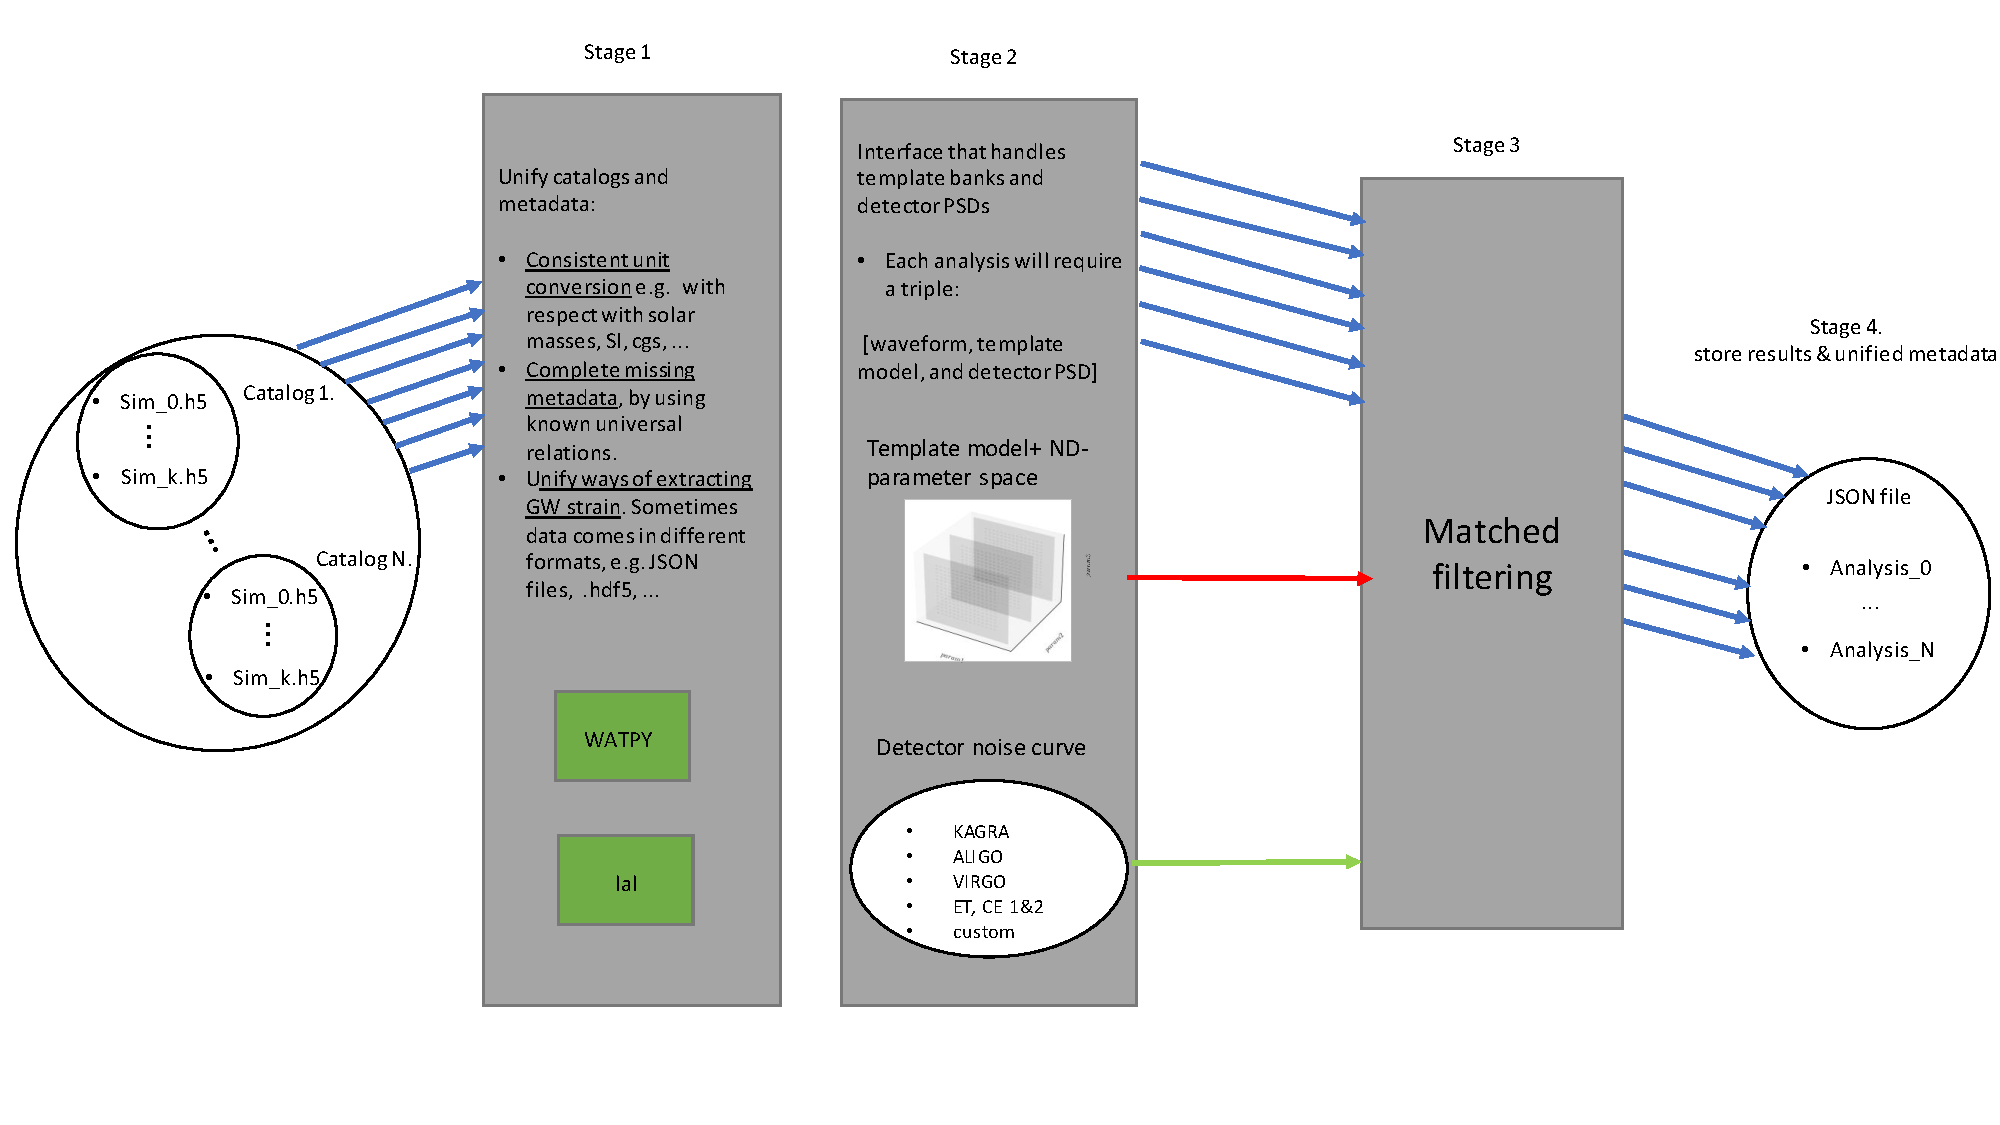
\includegraphics[width=\textwidth, angle=0]{images/cat_search.pdf}
\captionsetup{width=0.8\textwidth}
\caption[Flowchart of matched filtering code for NR waveform catalogs]{Flowchart of matched filtering code for NR waveform catalogs. This diagram contains the schematics of the matched filtering code for NR waveform catalogs presented in section \ref{NR}. It is divided into four stages, of which only stage 3 employs equation \ref{pul}. Stages 1 and 2 depict the waveform extraction done through python packages like WATPY and LAL, template bank generation and conditioning of detector sensitivity curves, and stage 4 for results and metadata storage.}
\label{fig:19}
\end{center}
\end{sidewaysfigure}

\FloatBarrier


\section{The 2-dimensional finite monochromatic model}\label{2dsearch}

The following section will consider a template model that only accounts for the most dominant frequency and duration of a BNS postmerger GW. Hence, it will be constructed by using a sinusoidal wave with constant amplitude and frequency and a rectangular window to define its finite duration 

%\begin{equation}\label{eq:19}
%q_{_{_{A, f, \phi_0, t_{0}, d}}}(t) =A \cdot sin(2\pi f t + \phi_0) \cdot \Pi_{t_{0},t_{0} + d}(t)=
%\begin{cases} 
%      0 & t<t_{0} \\
%      A \cdot sin(2\pi f t + \phi_0) & t_{0} \leq t\leq t_{0}+d \\
%      0 & t>t_{0}+d
%   \end{cases}
%\end{equation}

\begin{equation}\label{eq:19}
q_{_{_{A, f, \phi_0, t_{0}, d}}}(t) =A \cdot sin(2\pi f t + \phi_0) \cdot \Pi_{t_{0},t_{0} + d}(t)
\end{equation}


\begin{equation}\label{eq:18}
\Pi_{_{_{a,b}}}(t) = \theta(t-a)-\theta(t-b) = 
\begin{cases} 
      0 & a<t \\
      1 & a \leq t\leq b \\
      0 & b>t
   \end{cases}
\end{equation}

Where $t_0$ is wave starting time, $t_0+d$ and $f$ its duration and frequency, and $A$ and $\phi$ its amplitude and phase. As seen in figure \ref{fig:7}, matched filtering algorithm allows us to find the optimal values for amplitude, phase, and timeshift $A_{opt}$, $\phi_{opt}$ and $t_{0_{opt}}$, such that the template model \ref{eq:19}, can be written as

\begin{equation}\label{eq:20}
q_{_{_{f,d}}}(t) =
\begin{cases} 
      0 & t<t_{0_{opt}} \\
      A_{opt} \cdot sin(2\pi f t + \phi_{0_{opt}}) & t_{0_{opt}} \leq t\leq t_{0_{opt}}+d \\
      0 & t>t_{0_{opt}}+d
   \end{cases}
%\label{eq_uk}.
\end{equation}

The recovered SNR equation \ref{pul} can be written in terms of the 2-dimensional bank of templates \ref{eq:20}

\begin{equation}\label{eq:21}
\rho_{_{_{f,d}}} = \frac{\langle h, q_{_{_{f,d}}}\cdot e^{i(2\pi \tau+\phi)}\rangle \bigg\rvert_{\phi =\phi_{opt},\tau =\tau_{max}}}{\sqrt{\langle  q_{_{_{f,d}}},q_{_{_{f,d}}} \rangle}}
\end{equation}


For the sake of simplicity, in this thesis, template banks will be constructed in a uniform rectangular grid of 200 by 200 points, where the $f$-dimension varies from 500 to 3500 Hz, and the duration dimension varies between 0.1 milliseconds and $1.5 \cdot d_{postm}$ \ref{dp}. 

\begin{figure}[!htb]
\centering
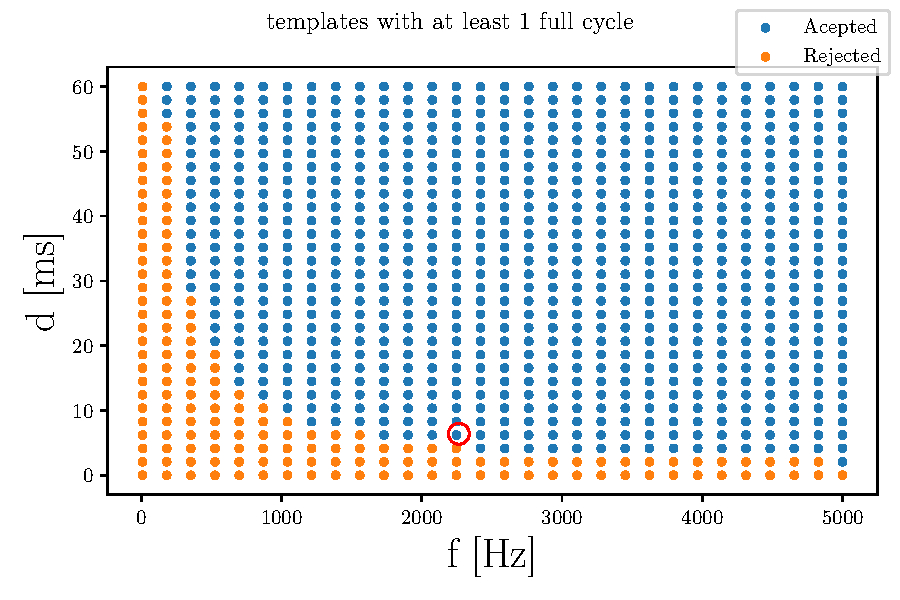
\includegraphics[scale=0.6]{images/Data_analysis/results/param_space.pdf}
\captionsetup{width=0.8\textwidth}
\caption[The parameter space of a finite monochromatic wave]{The parameter space of a finite monochromatic wave. This figure shows the parameter space of equation \ref{eq:19}. A mask is applied to discard combinations $(f,d)$ that generate templates with less than one wavelength (orange). The red circle shows the parameters used in figure \ref{fig:7}.}
\label{fig:11}
\end{figure}
\FloatBarrier

%However, notice that different algorithms address the problem of building template banks optimally, which is beyond the scope of what is presented here\cite{Allen_2021}.

Subsequently, the 2D recovered SNR \ref{eq:21}, normalized by the optimal SNR \ref{sopt}, will be computed at each point of the grid and will be represented as the third dimension using colormaps. 


The following figure shows how a \textit{Non-spinning equal mass BNS systems} may generate a postmerger signal that could be roughly described using a monochromatic model. Overlapping such a waveform against the template model \ref{eq:19} produces a colormap with a dominant peak in the region between 2-2.5 kHz at around 15ms. 

\begin{figure}[!htbp]
\begin{center}
\begin{minipage}[t]{0.5\linewidth}
\vspace{0pt}
%\raggedleft
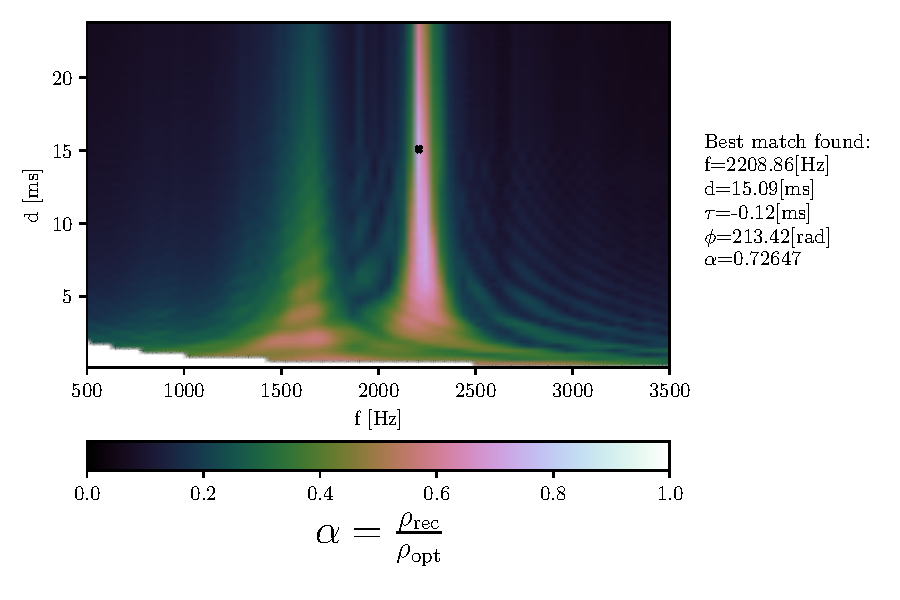
\includegraphics[scale=0.6,trim={2mm 0 35mm 0},clip]{images/Data_analysis/results/2D_grid_1.pdf}
\end{minipage}%
\begin{minipage}[t]{0.5\linewidth}
\vspace{20pt}
%\raggedright
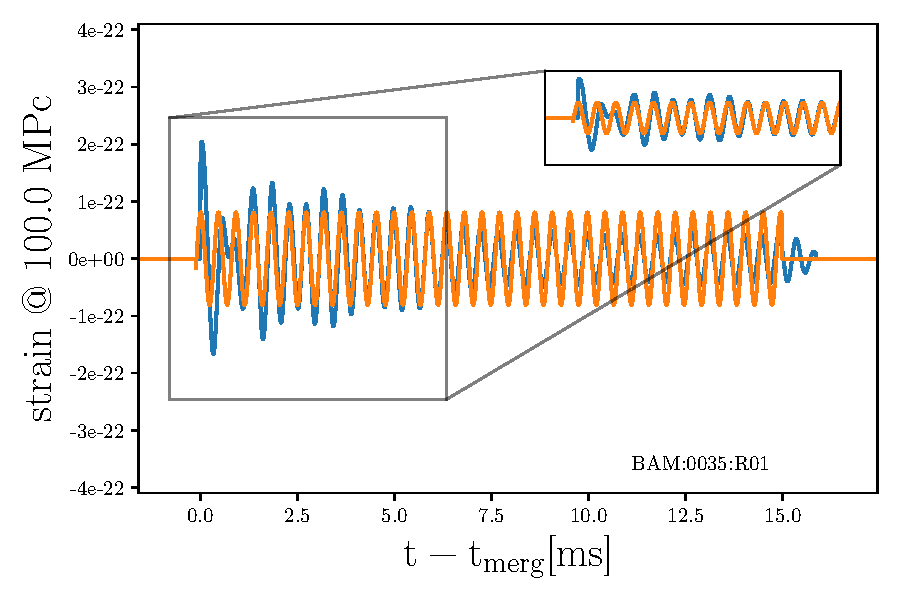
\includegraphics[scale=0.45]{images/Data_analysis/results/2D_grid_2.pdf}
\end{minipage}
\captionsetup{width=0.8\textwidth}
\caption[Equal mass BNS system's postmerger waveform and its best monochromatic match]{Equal mass BNS postmerger waveform and its best monochromatic match. This plot shows the recovered SNR \ref{eq:21} for the waveform BAM:0035:R01 of the CoRe BNS catalog \cite{Dietrich:2018phi} and the template model \ref{eq:19}. The best matching parameters are $f=2208.86$ Hz and $d=15.09$ ms.}
\label{eqmass}
\end{center}
\end{figure}

\FloatBarrier

Below, a few other example waveforms will be overlapped against the template model \ref{eq:19} to depict how the matched filtering algorithm, may not recover accurately the frequency and duration of other more complex BNS postmerger waveforms in the catalogs described in section \ref{NR}.
 

\textit{High mass ratio BNS systems}, i.e., $q=m_1/m_2>1.6$ may show a dominant peak in the low duration-low frequency region. Notice that there are other subdominant structures in the colormap around 2.5 kHz, belonging to templates that would match the low amplitude portion of the postmerger tail.

\begin{figure}[!htbp]
\begin{center}
\begin{minipage}[t]{0.5\linewidth}
\vspace{0pt}
%\raggedleft
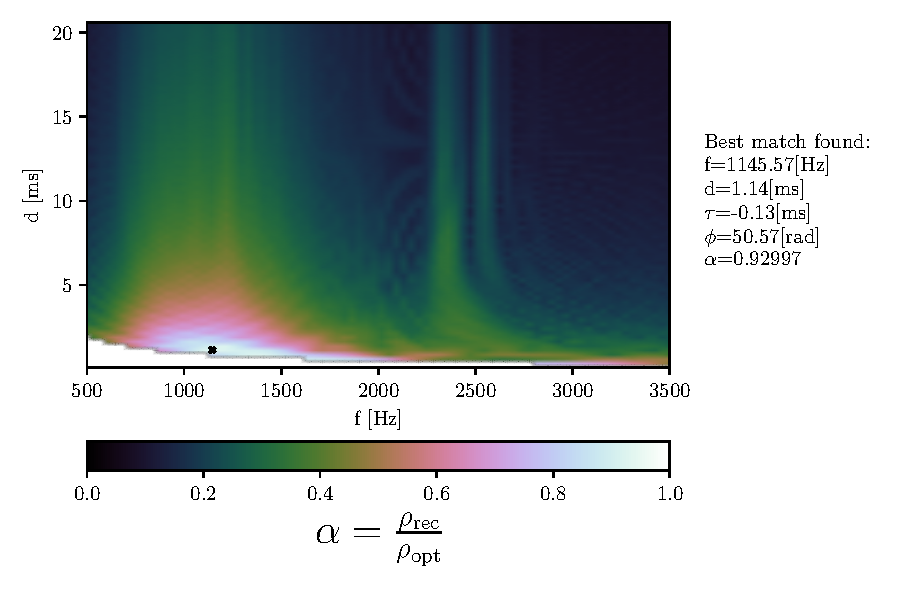
\includegraphics[scale=0.6,trim={2mm 0 35mm 0},clip]{images/Data_analysis/results/2D_grid_3.pdf}
\end{minipage}%
\begin{minipage}[t]{0.5\linewidth}
\vspace{20pt}
%\raggedright
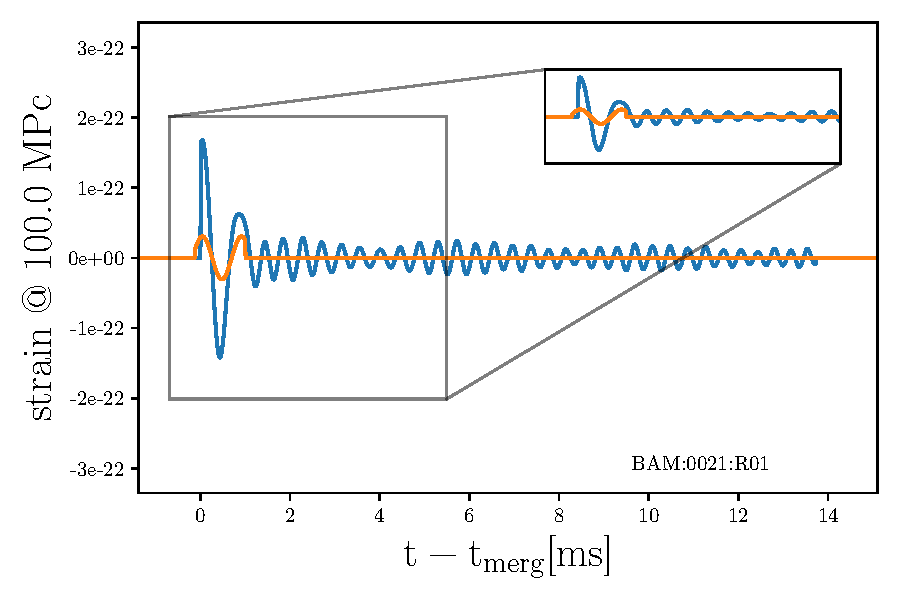
\includegraphics[scale=0.45]{images/Data_analysis/results/2D_grid_4.pdf}
\end{minipage}
\captionsetup{width=0.8\textwidth}
\caption[High mass ratio BNS system's postmerger waveform and its best monochromatic match]{High mass ratio BNS postmerger waveform and its best monochromatic match. This plot shows the recovered SNR \ref{eq:21} for the waveform BAM:0021:R01 of the CoRe BNS catalog \cite{Dietrich:2018phi} and the template model \ref{eq:19}. The best matching parameters are $f=1145.57$ Hz and $d=1.14$ ms.}
\end{center}
\end{figure}

\FloatBarrier


\newpage

\textit{Spinning BNS systems} i.e. $\chi_{eff}>0.2$(see equation \ref{chieff}) have a more complex frequency evolution. The colormap shows two regions of SNR excess: a wide one ranging from 1-2.5 kHz and duration below 5ms, and the other between 3-3.5 kHz with a peak duration around half waveform's duration $d_{postm}$. Notice that both regions have similar amounts of SNR recovery, so even though this example waveform prefers a long high frequency monochromatic segment, in some other cases, it may be a short, low frequency one.

\begin{figure}[!htbp]
\begin{center}
\begin{minipage}[t]{0.5\linewidth}
\vspace{0pt}
%\raggedleft
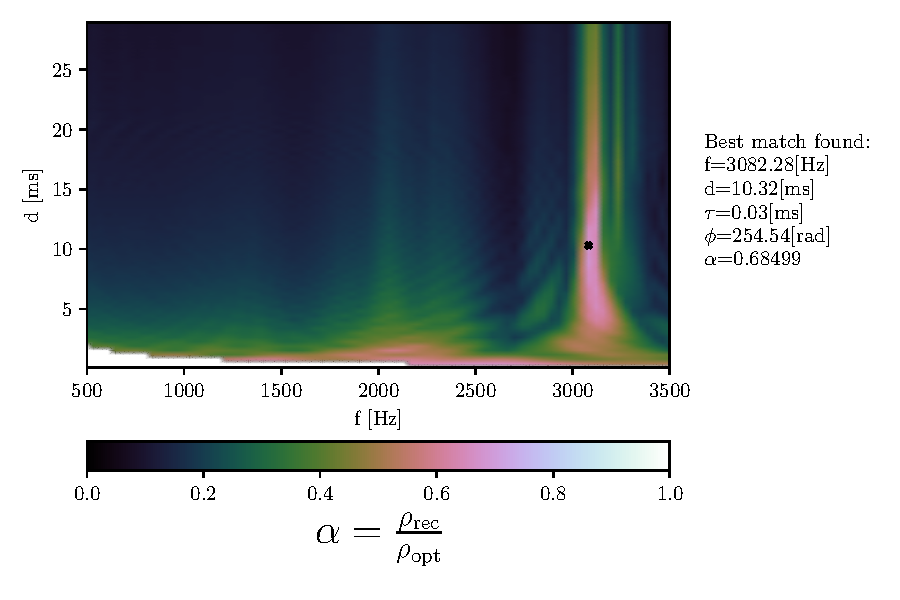
\includegraphics[scale=0.6,trim={2mm 0 35mm 0},clip]{images/Data_analysis/results/2D_grid_5.pdf}
\end{minipage}%
\begin{minipage}[t]{0.5\linewidth}
\vspace{20pt}
%\raggedright
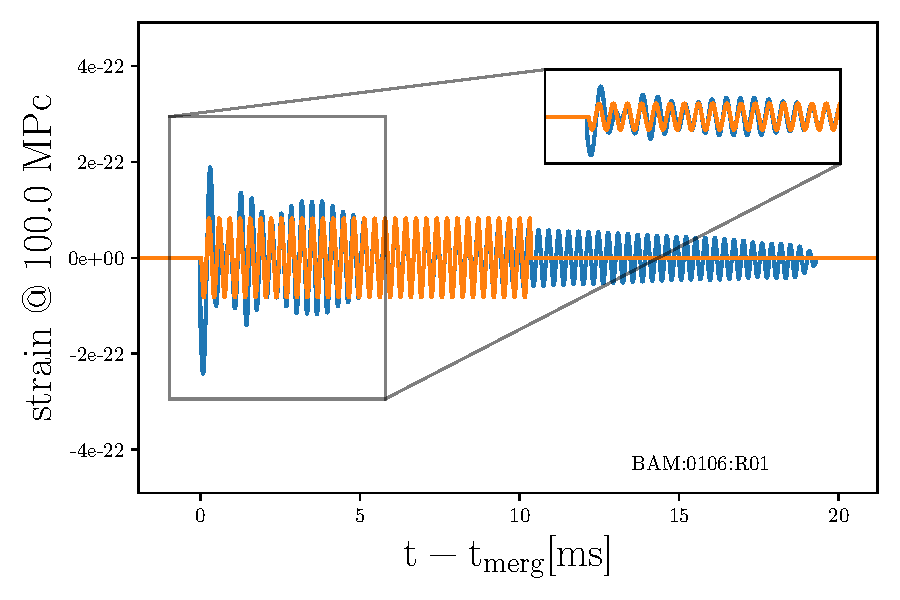
\includegraphics[scale=0.45]{images/Data_analysis/results/2D_grid_6.pdf}
\end{minipage}
\captionsetup{width=0.8\textwidth}
\caption[Spinning BNS system's postmerger waveform and its best monochromatic match]{Spinning BNS postmerger waveform and its best monochromatic match. This plot shows the recovered SNR \ref{eq:21} for the waveform BAM:0106:R01 of the CoRe BNS catalog \cite{Dietrich:2018phi} and the template model \ref{eq:19}. The best matching parameters are $f=3082.28$ Hz and $d=10.32$ ms.}
\label{spi}
\end{center}
\end{figure}

\FloatBarrier



\textit{Heavy BNS systems} i.e., $\delta=\frac{M_g}{M_{TOV}}>1.6$ may generate very short waveforms that contain at least one full high-frequency cycle(around 3 kHz) that can be easily fitted with a monochromatic wave.

\begin{figure}[!htbp]
\begin{center}
\begin{minipage}[t]{0.5\linewidth}
\vspace{0pt}
%\raggedleft
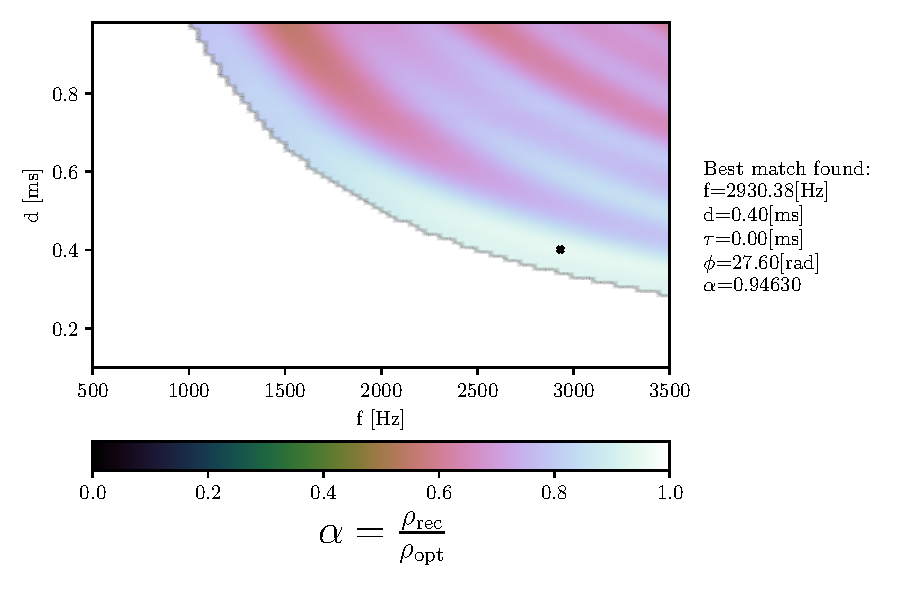
\includegraphics[scale=0.6,trim={2mm 0 35mm 0},clip]{images/Data_analysis/results/2D_grid_7.pdf}
\end{minipage}%
\begin{minipage}[t]{0.5\linewidth}
\vspace{20pt}
%\raggedright
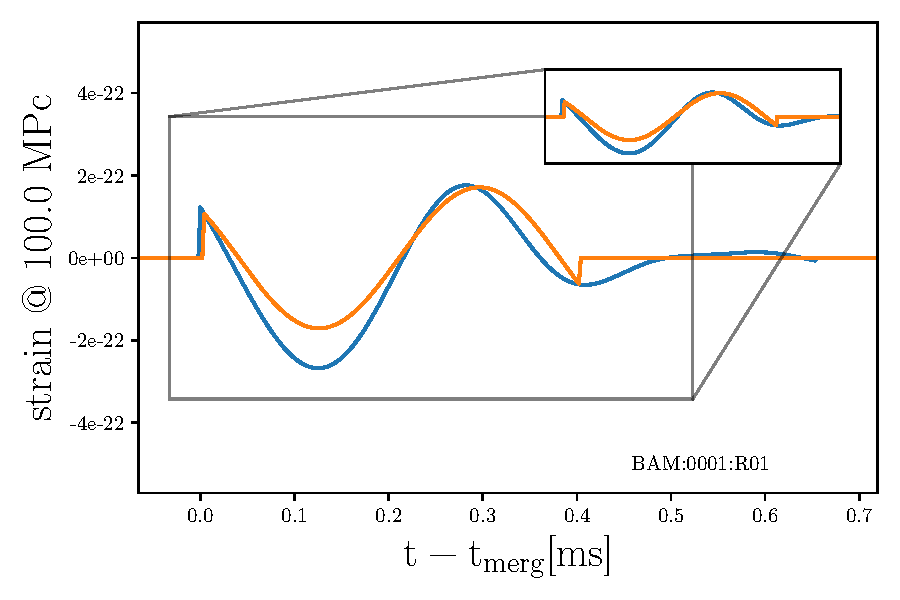
\includegraphics[scale=0.45]{images/Data_analysis/results/2D_grid_8.pdf}
\end{minipage}
\captionsetup{width=0.8\textwidth}
\caption[Heavy BNS system's postmerger waveform and its best monochromatic match]{Heavy BNS system's postmerger waveform and its best monochromatic match. This plot shows the recovered SNR \ref{eq:21} for the waveform BAM:0001:R01 of the CoRe BNS catalog \cite{Dietrich:2018phi} and the template model \ref{eq:19}. The best matching parameters are $f=2930$ Hz and $d=0.40$ ms.}
\end{center}
\end{figure}

\FloatBarrier
 

\newpage
\textit{Highly eccentric BNS systems} i.e., $e>0.4$, show a wide structure on the low-frequency side that dominates the colormap, resulting in short best matches, similar to high mass ratio waveforms


\begin{figure}[!htbp]
\begin{center}
\begin{minipage}[t]{0.5\linewidth}
\vspace{0pt}
%\raggedleft
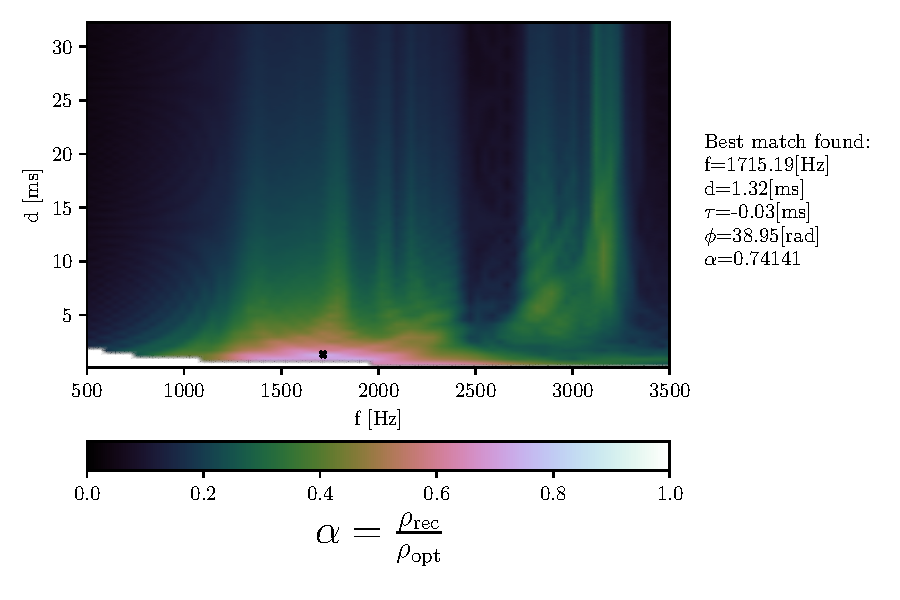
\includegraphics[scale=0.6,trim={2mm 0 35mm 0},clip]{images/Data_analysis/results/2D_grid_9.pdf}
\end{minipage}%
\begin{minipage}[t]{0.5\linewidth}
\vspace{20pt}
%\raggedright
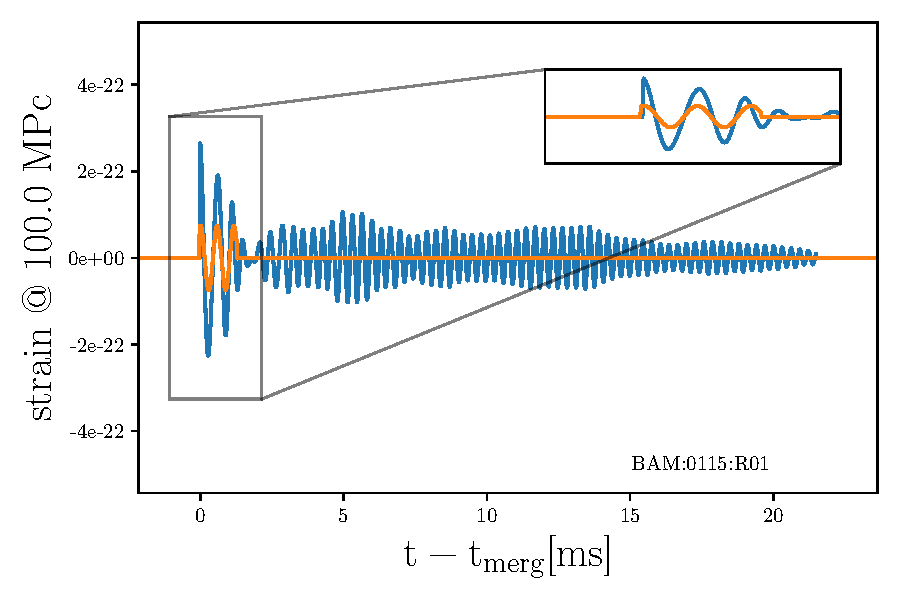
\includegraphics[scale=0.45]{images/Data_analysis/results/2D_grid_10.pdf}
\end{minipage}
\captionsetup{width=0.8\textwidth}
\caption[Eccentric BNS system's postmerger waveform and its best monochromatic match]{Eccentric BNS system's postmerger waveform and its best monochromatic match. This plot shows the recovered SNR \ref{eq:21} for the waveform BAM:0115:R01 of the CoRe BNS catalog \cite{Dietrich:2018phi} and the template model \ref{eq:19}. The best matching parameters are $f=1715.19$ Hz and $d=1.32$ ms.}
\end{center}
\end{figure}

\FloatBarrier


\textit{Simulations of equal mass BNS systems} that consider viscous hydrodynamics generate waveforms with a stronger amplitude modulation than the example shown in figure \ref{eqmass}. However, such effects do not change significantly the colormaps, which also have a dominant peak in the region between 2-3 kHz.


\begin{figure}[!htbp]
\begin{center}
\begin{minipage}[t]{0.5\linewidth}
\vspace{0pt}
%\raggedleft
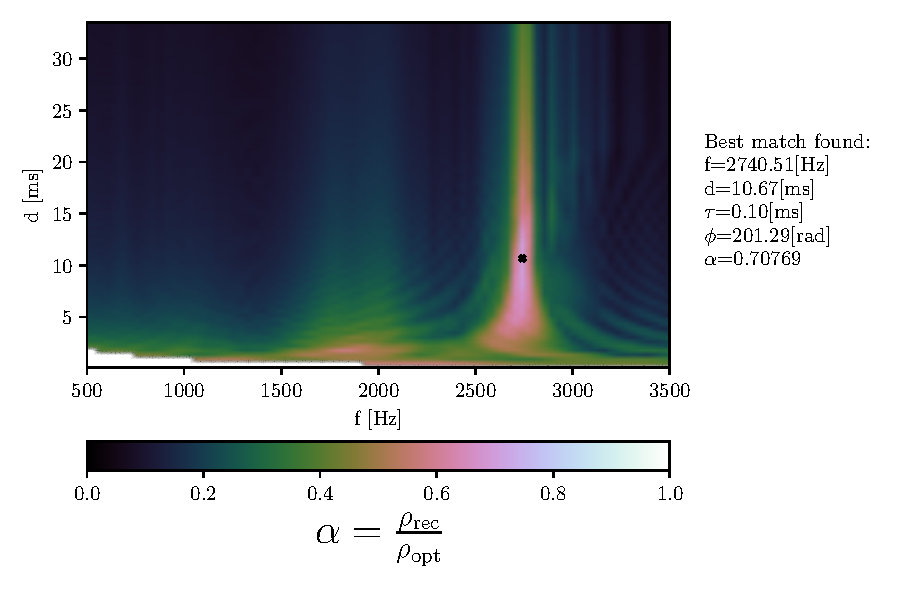
\includegraphics[scale=0.6,trim={2mm 0 35mm 0},clip]{images/Data_analysis/results/2D_grid_11.pdf}
\end{minipage}%
\begin{minipage}[t]{0.5\linewidth}
\vspace{20pt}
%\raggedright
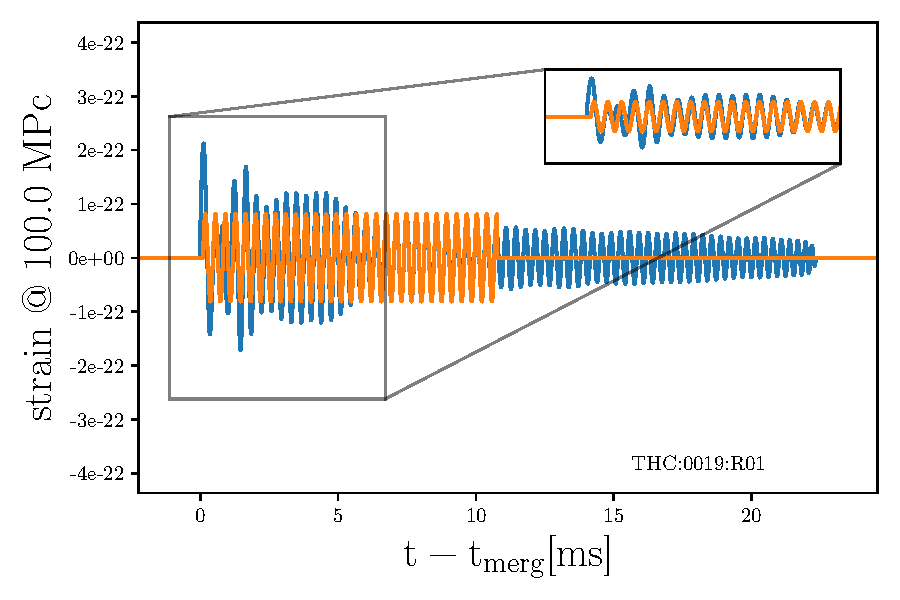
\includegraphics[scale=0.45]{images/Data_analysis/results/2D_grid_12.pdf}
\end{minipage}
\captionsetup{width=0.8\textwidth}
\caption[The impacts of microphyscis in the postmerger's best monochromatic match]{The impacts of microphyscis in the postmerger's best monochromatic match. This plot shows the recovered SNR \ref{eq:21} for the waveform THC:0019:R01 of the CoRe BNS catalog \cite{Dietrich:2018phi} and the template model \ref{eq:19}. The best matching parameters are $f=2740.61$ Hz and $d=10.67$ ms.}
\end{center}
\end{figure}

\FloatBarrier



Since eccentric, high mass ratio, or spinning BNS systems may generate waveforms that are challenging for the monochromatic model \ref{eq:19}. We can avoid searching in the low frequency region with a different question that slightly modifies the target of the search:

Original question$\rightarrow$" Which parameters f and d would produce the monochromatic wave that recovers most of the signal-to-noise ratio?"

New question$\rightarrow$" Which parameters f and d would produce the monochromatic wave that recovers most of the signal-to-noise ratio and contain more than n oscillations?"


Modifying the question in such a way would increase the number of rejected points lying on the orange region(see figure \ref{fig:11}) and get rid of the loud low-frequency structure dominating the colormaps, which is related to oscillations right after $t_{merg}$.


\begin{itemize}[leftmargin=*]


\item High mass ratio waveform, using constraint n=15.

\begin{figure}[!htbp]
\begin{center}
\begin{minipage}[t]{0.5\linewidth}
\vspace{0pt}
%\raggedleft
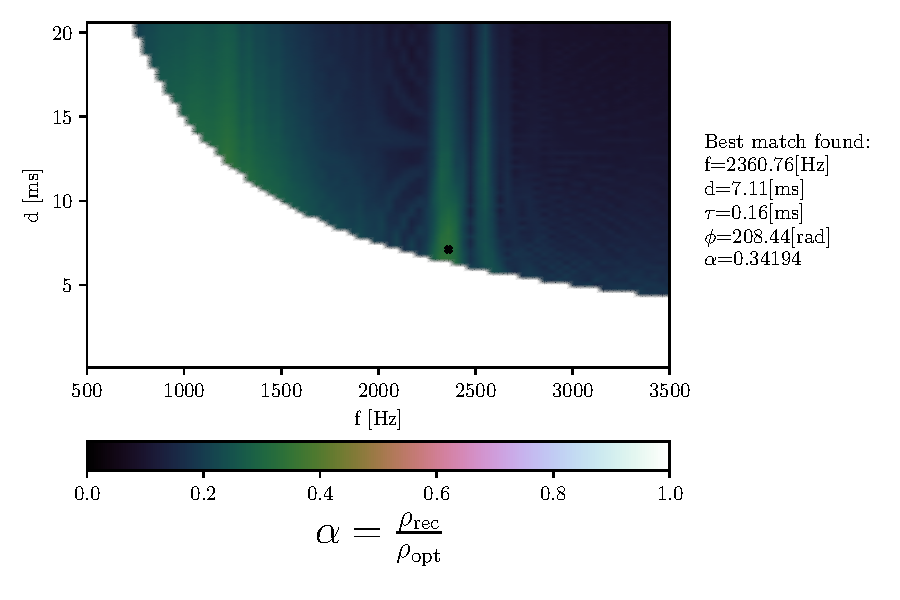
\includegraphics[scale=0.6,trim={2mm 0 35mm 0},clip]{images/Data_analysis/results/2D_grid_13.pdf}
\end{minipage}%
\begin{minipage}[t]{0.5\linewidth}
\vspace{20pt}
%\raggedright
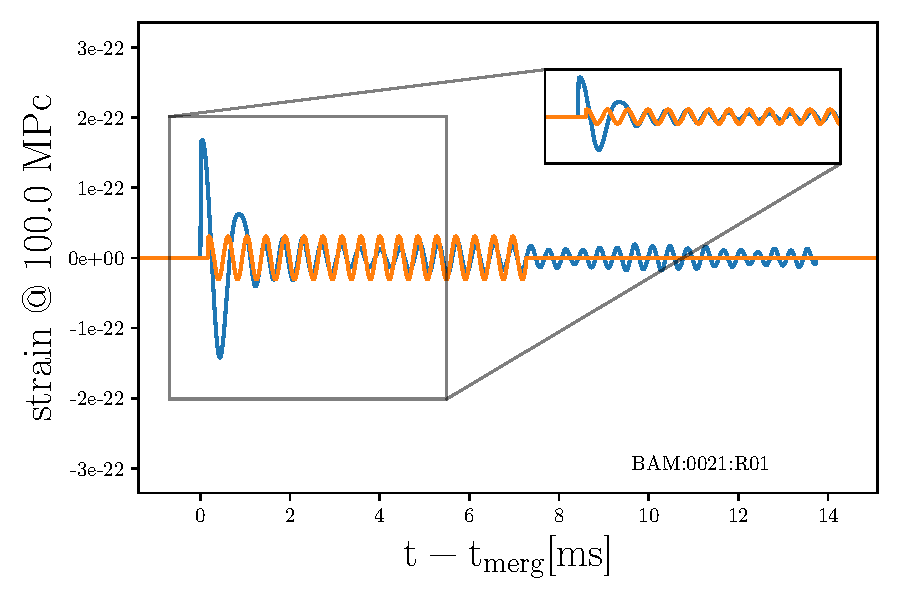
\includegraphics[scale=0.45]{images/Data_analysis/results/2D_grid_14.pdf}
\end{minipage}
\captionsetup{width=0.8\textwidth}
\caption[Duration constraint for high mass ratio waveform]{Duration constraint for high mass ratio waveform. This plot shows the recovered SNR \ref{eq:21} for the waveform BAM:0021:R01 of the CoRe BNS catalog \cite{Dietrich:2018phi} and the template model \ref{eq:19}. The duration constraint of at least n=15 oscillations is imposed using a different mask on parameter space.}
\end{center}
\end{figure}

\FloatBarrier


\item Highly eccentric waveform, using constraint n=15.

\begin{figure}[!htbp]
\begin{center}
\begin{minipage}[t]{0.5\linewidth}
\vspace{0pt}
%\raggedleft
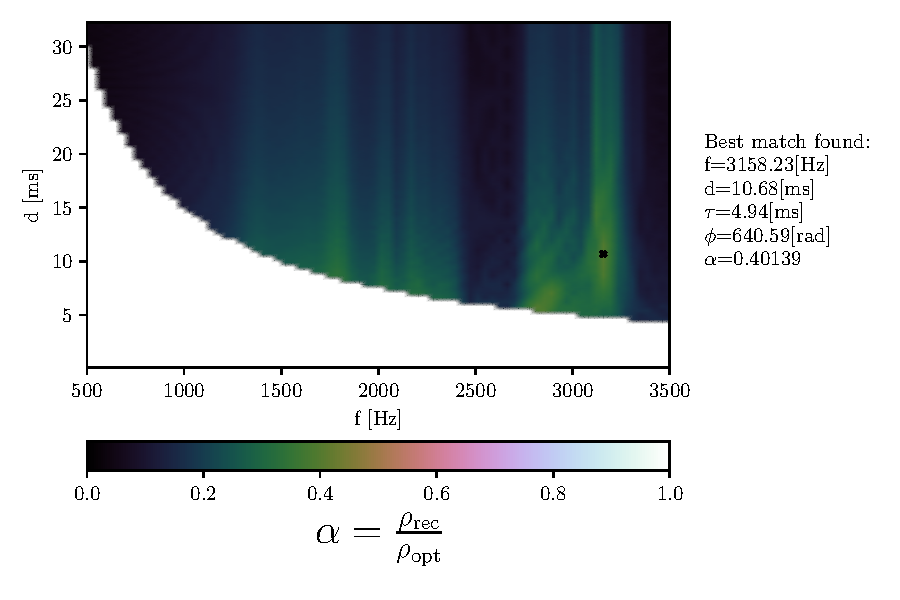
\includegraphics[scale=0.6,trim={2mm 0 35mm 0},clip]{images/Data_analysis/results/2D_grid_15.pdf}
\end{minipage}%
\begin{minipage}[t]{0.5\linewidth}
\vspace{20pt}
%\raggedright
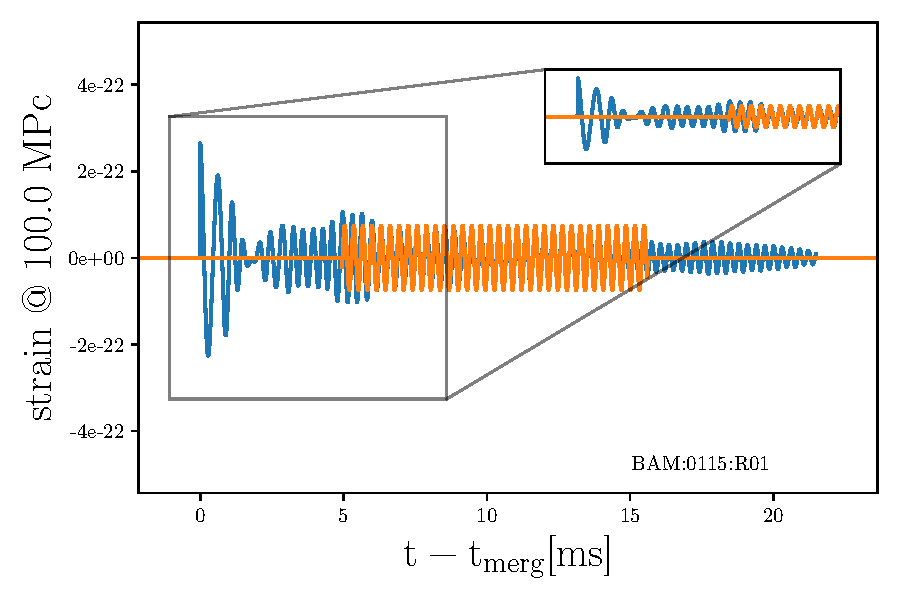
\includegraphics[scale=0.45]{images/Data_analysis/results/2D_grid_16.pdf}
\end{minipage}
\captionsetup{width=0.8\textwidth}
\caption[Duration constraint for highly eccentric waveform]{Duration constraint for highly eccentric waveform. This plot shows the recovered SNR \ref{eq:21} for the waveform BAM:0115:R01 of the CoRe BNS catalog \cite{Dietrich:2018phi} and the template model \ref{eq:19}. The duration constraint of at least n=15 oscillations is imposed using a different mask on parameter space.}
\end{center}
\end{figure}

\FloatBarrier

\end{itemize}


Even though imposing such constraints on parameter space might help to recover the template frequency and duration, using such a method in real GW searches seems unfeasible since the GW signal's starting time and duration are unknown.

\newpage
\section{How well can the monochromatic model recover signals in the catalog?}

The fact that one can find postmerger waveforms in the dataset \ref{NR} where a finite monochromatic model produces the results shown in figure \ref{eqmass} leads us to ask how the model \ref{eq:19} would perform across the whole waveform dataset. 
 
This section will use the infrastructure described in figure \ref{fig:19} to analyze iteratively the whole dataset of 220 waveforms (see section \ref{NR}). Using the finite monochromatic template model \ref{eq:19} equation \ref{eq:21} for computing the maximum recovered SNR takes the form



\begin{equation}\label{eq:22}
\rho_{_{_{rec}}} := \rho^j_{_{_{f,d}}} = \frac{\langle h^j, q_{_{_{f,d}}}\cdot e^{i(2\pi \tau+\phi)}\rangle \bigg\rvert_{\phi =\phi_{opt},\tau =\tau_{max}}}{\sqrt{\langle  q_{_{_{f,d}}},q_{_{_{f,d}}} \rangle}}
\end{equation}


Let $f_{best}$ and $d_{best}$ be the parameters of the best matching template \ref{eq:20} that recover the maximum SNR \ref{eq:22}  for a given waveform $h^j$ in the catalog. Several 2D planes like $\rho_{opt}$-$\alpha$, $\rho_{opt}$-$\beta$ and $\rho_{opt}$-$\gamma_{wei}$ will describe at the end of the analysis the characteristics of the waveform dataset based on SNR recovery and parameter estimation accuracy. Where $\alpha$ is given by equation \ref{ff} and,

\begin{equation}
\beta=d_{best}/d_{postm},
\end{equation}

\begin{equation}
\gamma_{wei}=f_{best}/f_{wei}.
\end{equation}

Let us start by imposing the following color coding for different regions of the $\rho_{opt}$-$\alpha$ plane, and a threshold optimal SNR \ref{sopt} of 8 at 100 MPc (see \cite[section 3]{https://doi.org/10.48550/arxiv.2109.09882}).


\begin{figure}[hbt!]
\begin{center}
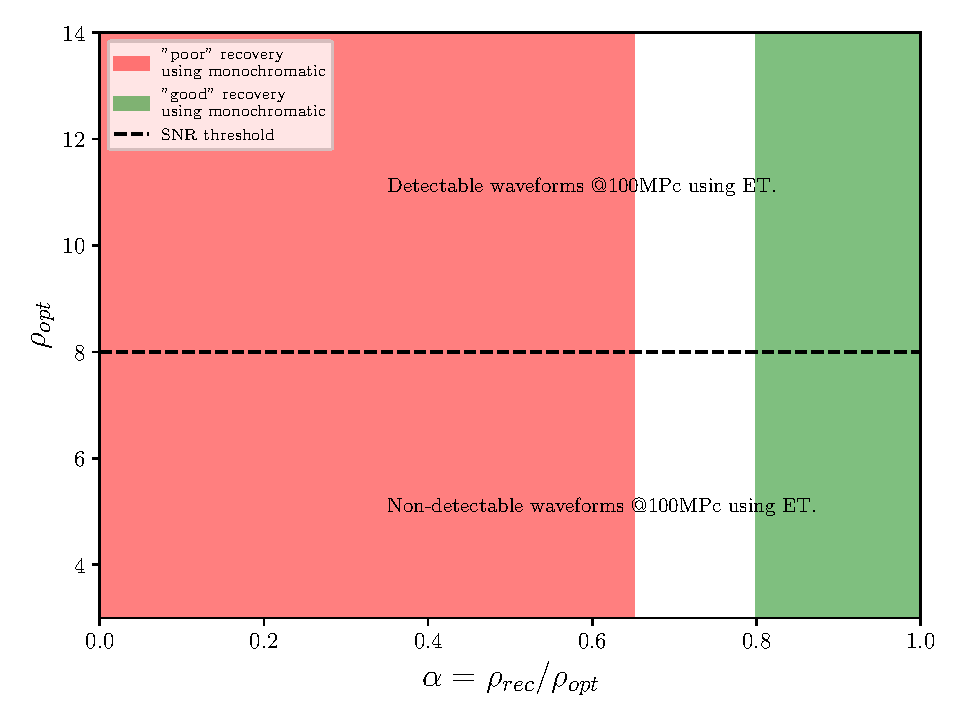
\includegraphics[width=0.8\textwidth, angle=0]{images/Data_analysis/results/schematics.pdf}
\captionsetup{width=0.8\textwidth}
\caption[Detectablity and features of a waveform catalog]{Detectablity and features of a waveform catalog. This figure depicts the way the dataset will be divided and characterized in terms of optimal SNR \ref{sopt}, and the SNR ratio $\alpha=\rho_{rec}/\rho_{opt}$.}
\label{regions}
\end{center} 
\end{figure}

\FloatBarrier


The following interpretation can be given to waveforms in each of the four corners of figure \ref{regions}. Such coding will be key to separating groups of waveforms lying in one corner or the other.


\begin{itemize}
\item Upper left corner: signals that could be detected at 100 MPc, but the monochromatic model leaves a considerable margin of improvement.
\item Lower left corner: signals that would not be detected at 100 MPc, nor the monochromatic, represent a good model for them.
\item 
Upper right right: possibly detectable waveforms at 100MPc that require simple modeling.
\item 
Lower right corner: non-detectable waveforms at 100MPc that require simple modeling.
\end{itemize}


As we see in the following figure, overlapping every waveform in the dataset \ref{NR} will only produce SNR recoveries above 60\%. However, not all waveforms surpass the $\rho_{opt}=8$ threshold. Notice that all waveforms below $\alpha=0.65$ are marked with red crosses and waveforms with $\alpha=0.80$ with green ones.

\begin{figure}[hbt!]
\begin{center}
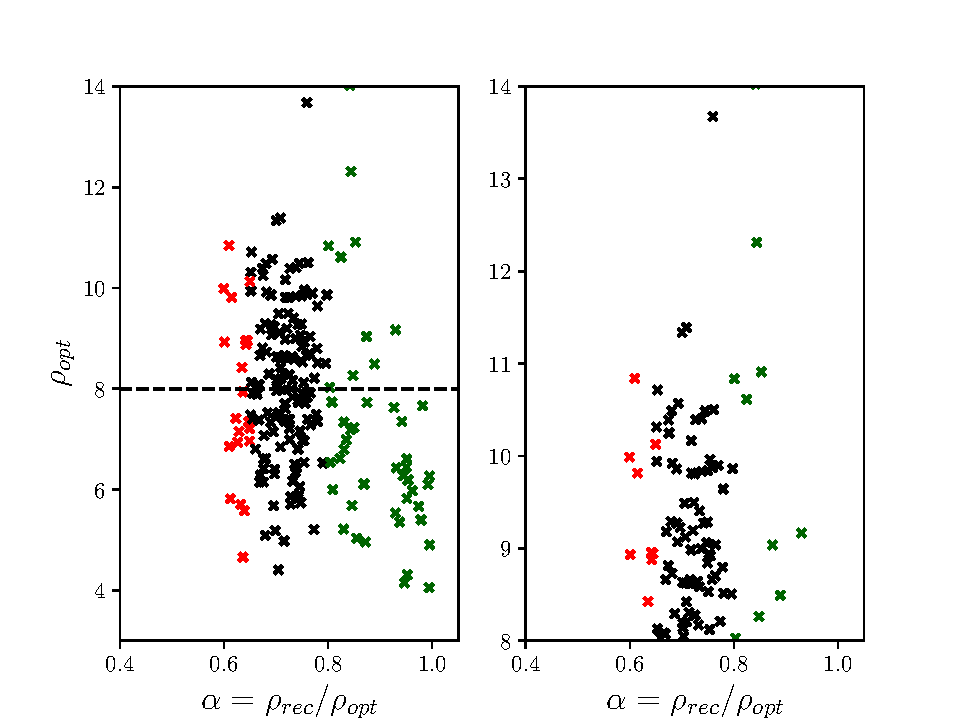
\includegraphics[width=\textwidth, angle=0]{images/Data_analysis/results/alpha_scatter.pdf}
\captionsetup{width=0.8\textwidth}
\caption[SNR recovery for the whole waveform dataset]{SNR recovery for the whole waveform dataset. This figure shows the $\rho_{opt}$-$\alpha$ plane to summarize the results obtained by overlapping all waveforms described in section \ref{NR} against the template model \ref{eq:20}. Results for the whole waveform dataset are shown on the left, and for waveforms above the $\rho_{opt}=8$ threshold on the right.}
\label{ascatter}
\end{center}
\end{figure}

\FloatBarrier

In what follows the the distribution of best matching parameters $f_{best}$, and $d_{best}$ alongside waveform properties like  $d_{wei}$, $f_{wei}$, and physical observables like $M=m_1+m_2$, $q=m_1/m_2$ and $\chi_{_{eff}}$ \ref{chieff} will be studied using histograms. We will color the histogram's bins according to $\alpha$ values to identify whether a certain type waveform shows up in one of the corners of  \ref{regions}, or rather the dataset is distributed uniformly in the $\rho_{_{opt}}$-$\alpha$ plane.

\newpage

The waveform distributions for $f_{wei}$, and $d_wei$, are shown below such that the whole waveform dataset (left) can be compared to the distribution of waveforms above the $\rho_{opt}=8$ threshold(right).

\begin{figure}[hbt!]
\begin{center}
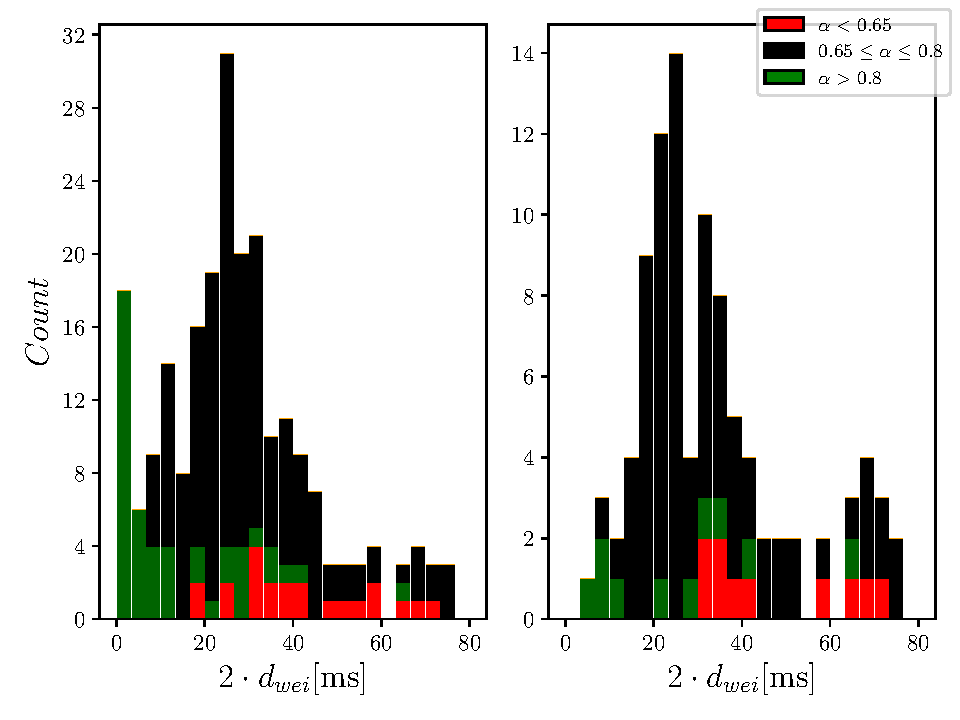
\includegraphics[width=0.6\textwidth, angle=0]{images/Data_analysis/results/alpha_dhist.pdf}
\captionsetup{width=0.8\textwidth}
\caption[Postmerger amplitude weighted durations in the waveform dataset]{Postmerger amplitude weighted durations in the waveform dataset. This figure shows the distribution of amplitude weighted durations (see equation \ref{dwei}) for all waveforms(left) and only waveforms above the optimal SNR threshold(right). The bar color is set according to the SNR recovery $\alpha$ as in figure \ref{ascatter}.}
\label{adhist}
\end{center}
\end{figure}



\begin{figure}[hbt!]
\begin{center}
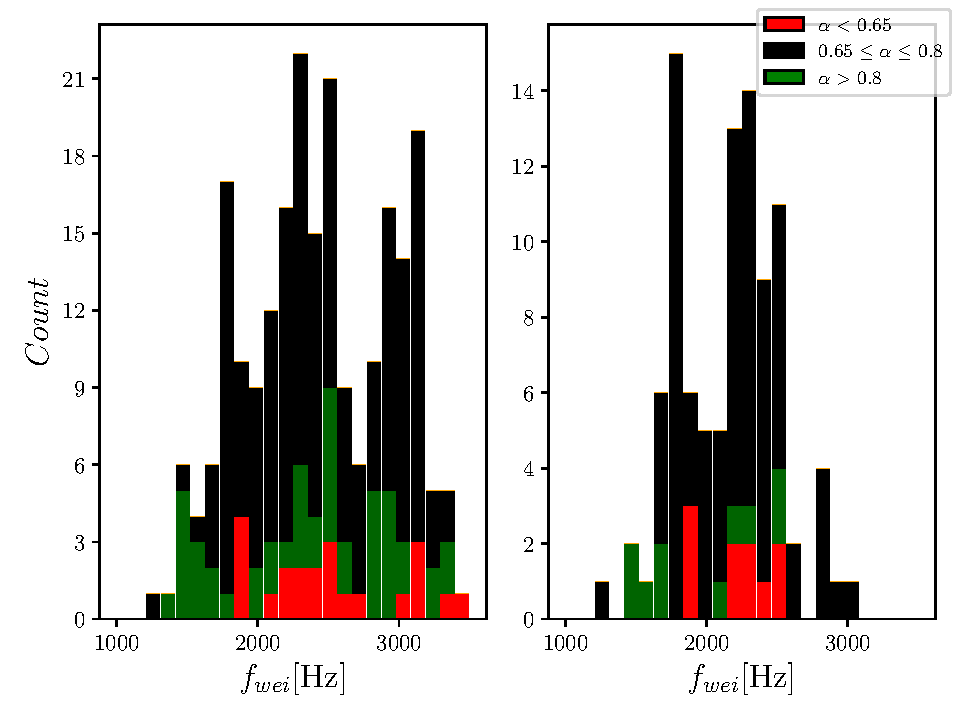
\includegraphics[width=0.6\textwidth, angle=0]{images/Data_analysis/results/alpha_fhist.pdf}
\captionsetup{width=0.8\textwidth}
\caption[Postmerger amplitude weighted frequencies in the postmerger waveform dataset]{Postmerger amplitude weighted frequencies in the waveform dataset. This figure shows the distribution of amplitude weighted frequencies (see equation \ref{fwei}) for all waveforms(left) and only waveforms above the optimal SNR threshold(right). The bar color is set according to the SNR recovery $\alpha$ as in figure \ref{ascatter}.}
\label{afhist}
\end{center}
\end{figure}
\FloatBarrier


Notice how transitioning from the whole dataset(left) to only above threshold waveforms(right) does two different things: It significantly reduces the tall green bar in figure \ref{adhist}. In addition, in figure \ref{afhist}, we see how most green bars disappear around the 3000Hz value in the weighted frequency histogram. Combining both plots, we can tell that the lower-right region in figure \ref{regions} contains many short waveforms with high average frequency.

Moreover, the red samples tell us how the monochromatic template model struggles to get more than 65\% of the optimal SNR for waveforms longer than 30 milliseconds. 


\newpage 

With regards to the parameters found for the best matching monochromatic template on each waveform of the catalog, we can use the histograms for the quantities  $\beta$ and $\gamma_{wei}$ 

\begin{figure}[hbt!]
\begin{center}
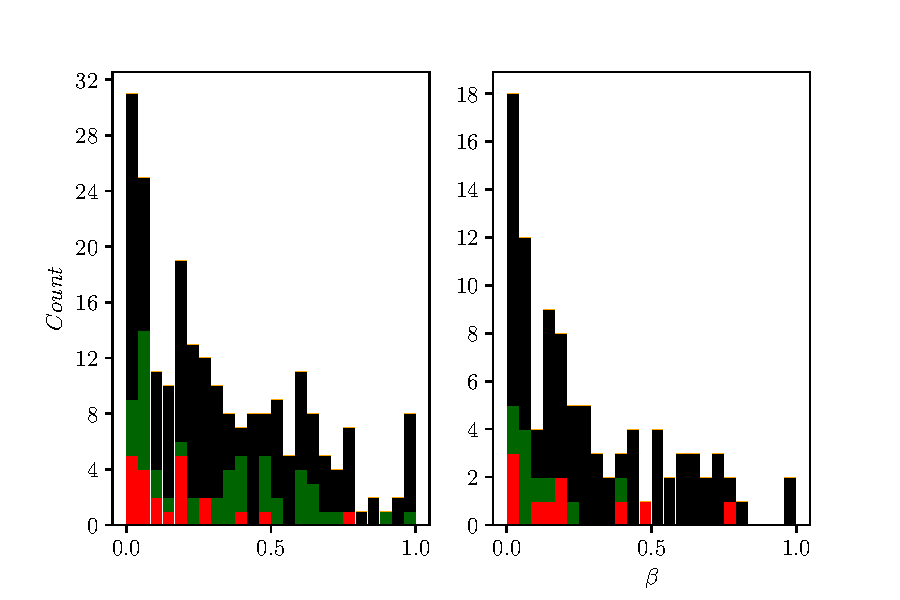
\includegraphics[width=0.6\textwidth, angle=0]{images/Data_analysis/results/alpha_betahist.pdf}
\captionsetup{width=0.8\textwidth}
\caption[Duration recovery in the postmerger waveform dataset]{Duration recovery in the postmerger waveform dataset. This figure shows the distribution of $\beta=d_{best}/d_{postm}$ for all waveforms(left) and only waveforms above the optimal SNR threshold(right). The bar color is set according to the SNR recovery $\alpha$ as in figure \ref{ascatter}.}
\label{abhist}
\end{center}
\end{figure}

\begin{figure}[hbt!]
\begin{center}
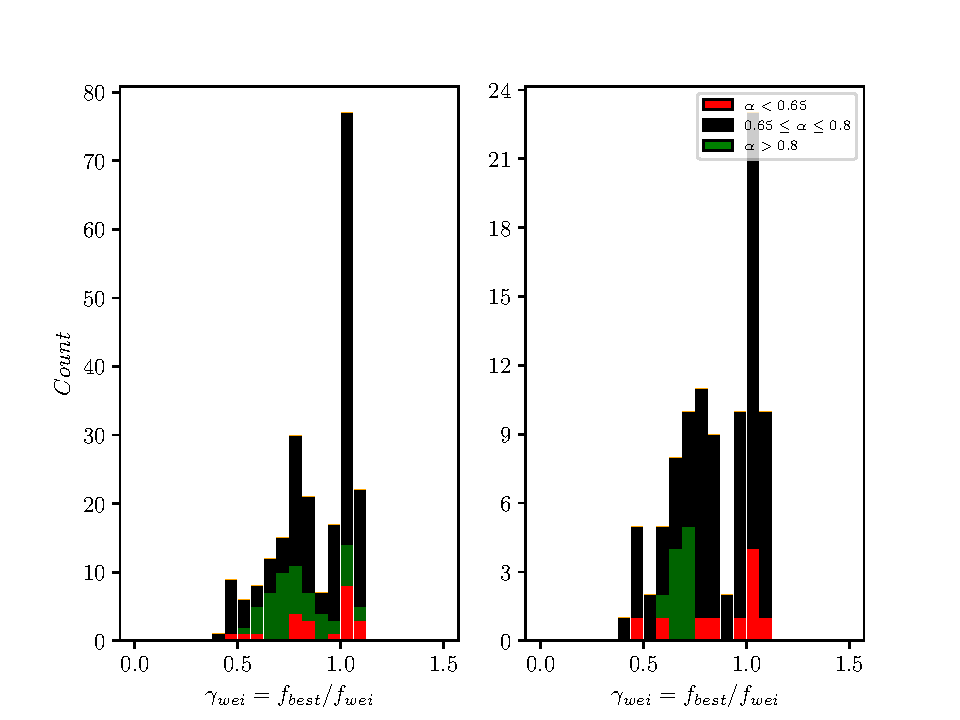
\includegraphics[width=0.6\textwidth, angle=0]{images/Data_analysis/results/alpha_gammahist.pdf}
\captionsetup{width=0.8\textwidth}
\caption[Frequency recovery in the postmerger waveform dataset]{Frequency recovery in the postmerger waveform dataset. This figure shows the distribution of $\gamma_{wei}=f_{best}/f_{wei}$ for all waveforms(left) and only waveforms above the optimal SNR threshold(right). The bar color is set according to the SNR recovery $\alpha$ as in figure \ref{ascatter}.}
\label{aghist}
\end{center}
\end{figure}
\FloatBarrier

Where the closer to 1.0, the better recovery of the signal duration and frequency one gets. Some waveforms in the green region recover the duration and weighted frequency well, but many green bars disappear as we go above the threshold. As previously seen, the red bars mainly belong to long waveforms, for which the monochromatic template performs very poorly recovering its length, regardless of whether the right weighted frequency was properly recovered, as the red bars seem very spread out in the $\gamma_{wei}$ histogram. 

\newpage

Finally, looking at physical observables like the system's total mass, mass ratio, and effective spin $\chi_{eff}$ we can check whether signal features like duration, recovery and their recovery in matched filtering runs are correlated to BNS properties.  

\begin{figure}[hbt!]
\begin{center}
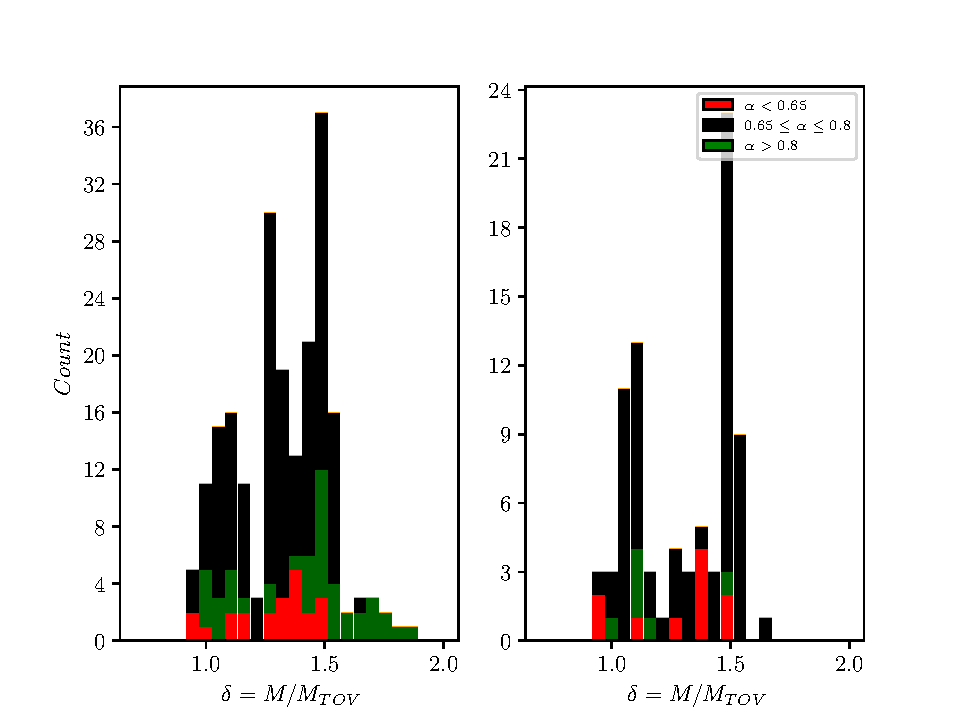
\includegraphics[width=0.6\textwidth, angle=0]{images/Data_analysis/results/alpha_deltahist.pdf}
\captionsetup{width=0.8\textwidth}
\caption[Total masses in the waveform dataset]{Total masses in the waveform dataset. This figure shows the distribution of $\delta=M/M_{TOV}$ for all waveforms(left) and only waveforms above the optimal SNR threshold(right). The bar color is set according to the SNR recovery $\alpha$ as in figure \ref{ascatter}.}
\label{adelhist}
\end{center}
\end{figure}

Counting the waveforms lying in the region where $\delta>1.6$, one can see that the green bars present in the whole dataset(left) disappear in the above threshold dataset(right). Such a set of signals can be identified as short high-frequency signals that belong to heavy systems. 

\begin{figure}[hbt!]
\begin{center}
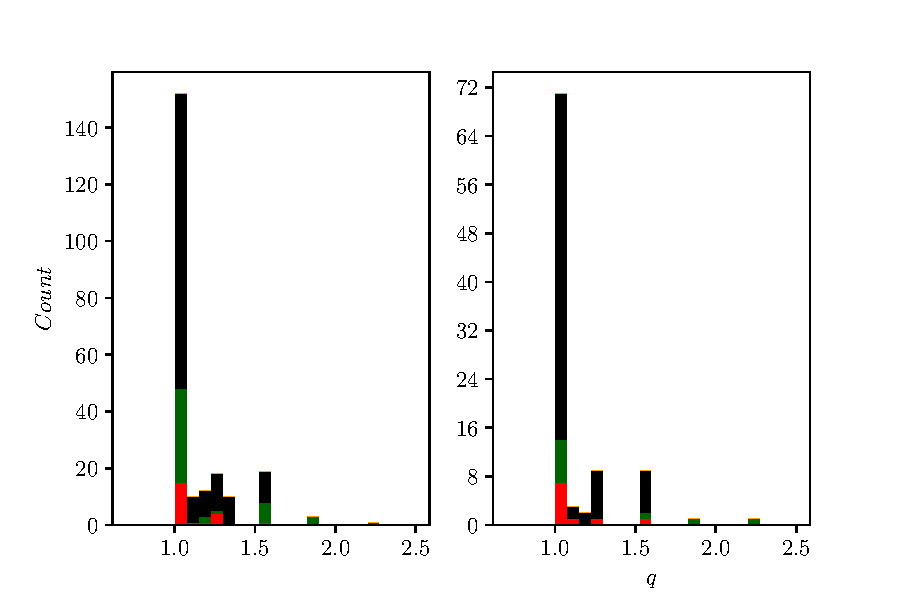
\includegraphics[width=0.6\textwidth, angle=0]{images/Data_analysis/results/alpha_qhist.pdf}
\captionsetup{width=0.8\textwidth}
\caption[Mass ratios in the waveform dataset]{Mass ratios in the waveform dataset. This figure shows the distribution of $q=m_1/m_2$ for all waveforms(left) and only waveforms above the optimal SNR threshold(right). The bar color is set according to the SNR recovery $\alpha$ as in figure \ref{ascatter}.}
\label{aqhist}
\end{center}
\end{figure}

As seen in figure \ref{aqhist}, the waveform dataset is dominated by equal mass waveforms. However, by looking at the few waveform samples with high mass ratio $q=m_1/m_2>1.6$, one can see that the green bars survive the threshold cut, which means they lie in the upper right region of plot \ref{aqhist}, making them good candidates for detection.
 

\newpage

Moreover, spinning BNS systems, i.e., $\chi_{eff}>0.2$ (see equation \ref{chieff}), are also a small subset in this catalog, as many waveforms come from non-spinning systems. Nevertheless, one can also see that the green bars survive the threshold cut, which means they lie in the upper right region of plot \ref{achihist}, making them good candidates for detection.

\begin{figure}[hbt!]
\begin{center}
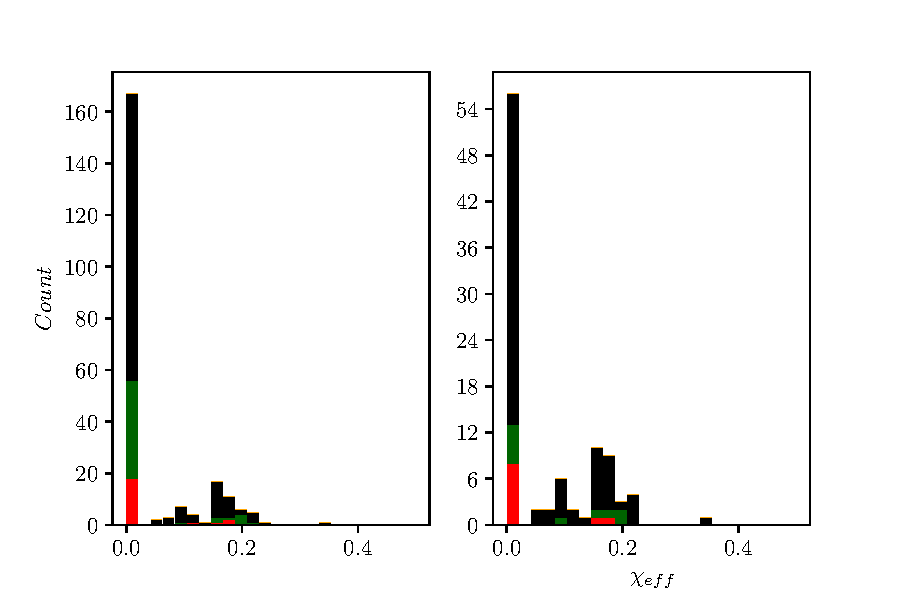
\includegraphics[width=0.6\textwidth, angle=0]{images/Data_analysis/results/alpha_chihist.pdf}
\captionsetup{width=0.8\textwidth}
\caption[Effective spins in the waveform dataset]{Effective spins in the waveform dataset. This figure shows the distribution of $\chi_{_{eff}}$ (see equation \ref{chieff}) for all waveforms(left) and only waveforms above the optimal SNR threshold(right). The bar color is set according to the SNR recovery $\alpha$ as in figure \ref{ascatter}.}
\label{achihist}
\end{center}
\end{figure}

\FloatBarrier


\subsection*{Findings}
Overall the finite monochromatic model with constant amplitude can recover between 65-98\% of the optimal signal-noise ratio \ref{sopt} for all waveforms in the dataset. In terms of SNR recovery, the most interesting cases, as seen in the following plot, are waveforms generated by equal mass non-spinning, highly eccentric, and heavy BNS coalescences. Notice how most short waveforms generated by heavy BNS systems lie below the optimal SNR threshold in the high SNR recovery region $\alpha>0.80$.

\begin{figure}[hbt!]
\begin{center}
\begin{tabular}{cc}
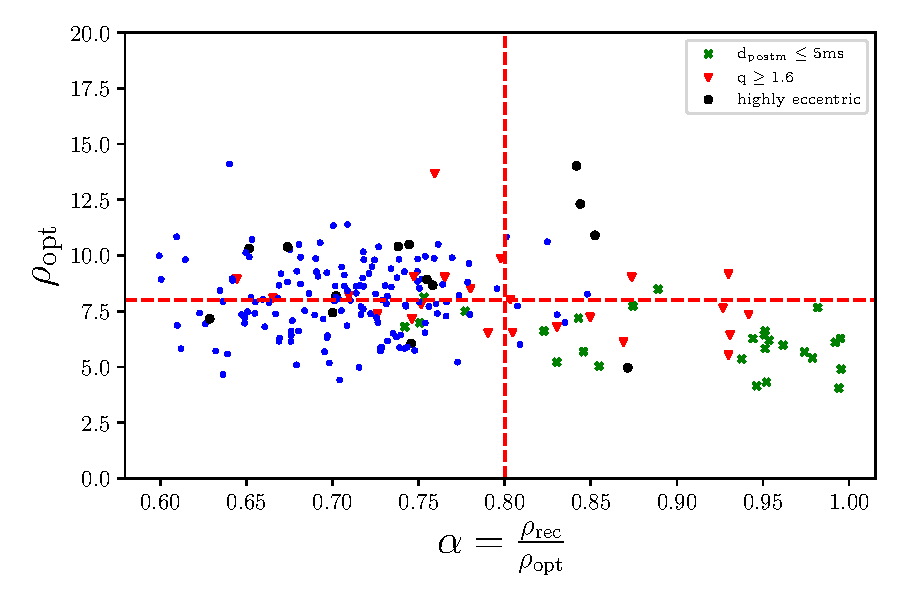
\includegraphics[width=0.55\textwidth, angle=0]{images/Data_analysis/results/alpha_sum0.pdf}
\end{tabular}
\captionsetup{width=0.8\textwidth}
\caption[SNR recovery summary]
{SNR recovery summary. This plot shows where different waveforms in the dataset lie in the $\rho_{opt}$-$\alpha$ plane. Notice that the region above $\alpha>0.7$ is populated mostly with either heavy systems (green), high mass ratio systems (red),  highly eccentric waveforms (black), and non-spinning equal mass waveforms (brown).}
\label{1}
\end{center}
\end{figure}
\FloatBarrier

\newpage


Moreover, even though waveforms generated by highly eccentric and high mass ratio BNS systems look like promissing candidates to be modeled using the monochromatic model \ref{eq:19}, the following two plots show that such a model does not recover accurately the postmerger's duration or main frequency.

\begin{figure}[hbt!]
\begin{center}
\begin{tabular}{cc}
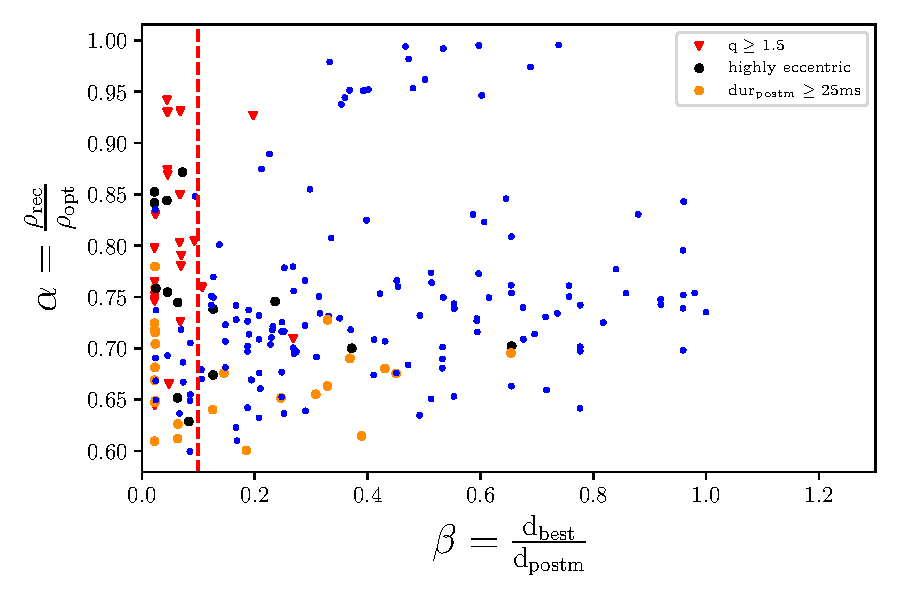
\includegraphics[width=0.6\textwidth, angle=0]{images/Data_analysis/results/alpha_sum1.pdf}
\end{tabular}
\captionsetup{width=0.8\textwidth}
\caption[Duration estimation summary]
{Duration estimation summary. This figure summarizes the search findings over the BNS waveform database according to \ref{regions}. It shows that highly eccentric (black), high mass ratio (red), and postmerger waveforms with a duration larger than 35 ms (orange) can not accurately recover the postmerger's duration. On the other hand, most of the equal mass waveforms (brown) lie in the region $\beta>0.2$}
\label{2}
\end{center}
\end{figure}

\FloatBarrier

\begin{figure}[hbt!]
\begin{center}
\begin{tabular}{cc}
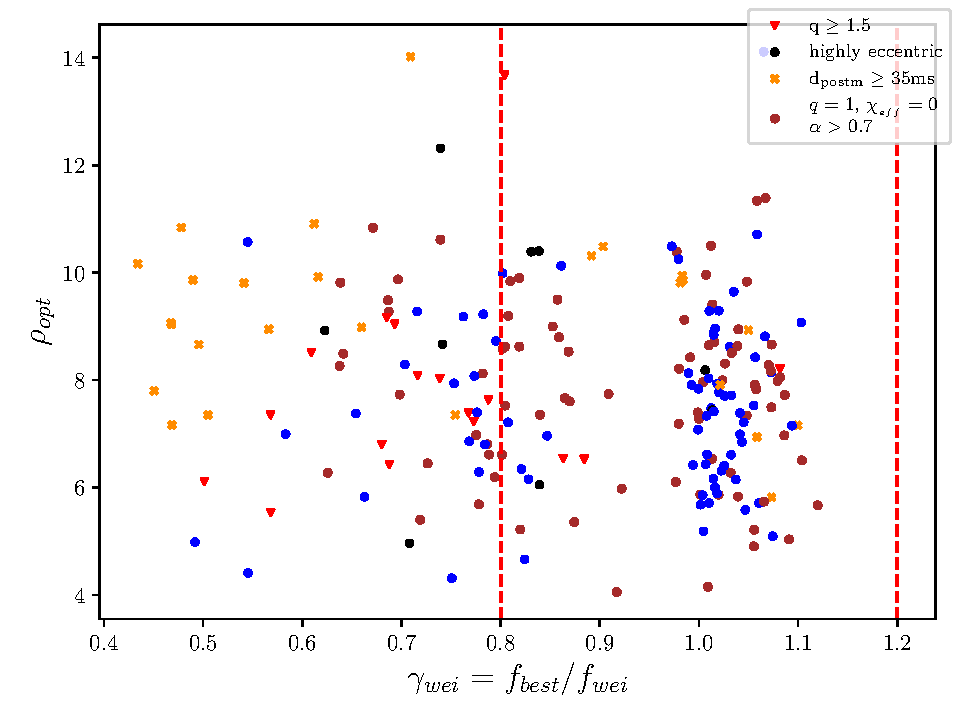
\includegraphics[width=0.6\textwidth, angle=0]{images/Data_analysis/results/alpha_sum2.pdf}
\end{tabular}
\captionsetup{width=0.8\textwidth}
\caption[Frequency estimation summary]
{Frequency estimation summary. This figure shows how the monochromatic model \ref{eq:19} can recover for non-spinning equal mass waveforms (brown) the postmerger's weighted frequency \ref{fwei}.
}
\label{3}
\end{center}
\end{figure}

\FloatBarrier

Finally, by looking at figures \ref{2} and \ref{3}, where brown dots represent the equal mass non-spinning binaries, one can see that the monochromatic model \ref{eq:20} can recover 70-80\% of the optimal SNR \ref{sopt} while reproducing the postmerger's duration and frequency more accurately than in the other cases.





\newpage
\section{Monochromatic models with modified amplitude envelopes}\label{zc-aenv}
One of the most characteristic features of a postmerger BNS signal is the first amplitude minimum after the merger which appears in every waveform of the dataset (see figure \ref{fig:9}). In this section, we will attempt to improve the finite monochromatic model with constant amplitude \ref{eq:20}, by adding a zero-crossing amplitude envelope to model such a feature. 

A wide variety of known functions could reproduce the first postmerger amplitude minimum. Nevertheless, we will only focus on a piecewise zero crossing linear function and a hyperbolic tangent function for the template envelope. 

\vspace{1cm}

\begin{itemize}
\item zero-crossing:
\begin{equation}\label{line}
Y0_{w, t_{min}}(t) =
\begin{cases} 
      1 &, t<t_{min}-\mathrm{\frac{width}{2}} \\
      \left( \frac{-2A}{\mathrm{width}} \right) \cdot (t- t_{min}) &, t_{min}-\mathrm{\frac{width}{2}} \leq t \leq t_{min}+\mathrm{\frac{width}{2}} \\
     -1 &, t>t_{0}+d
   \end{cases}
\end{equation}

\begin{equation}\label{tanh}
Y1_{\epsilon, t_{min}}(t) = A \cdot \tanh (\epsilon \cdot(t-t_{min}))
\end{equation}

Further, one could propose envelope models that, instead of crossing the zero line, touch it tangentially. This can be achieved by taking the absolute value of the piecewise linear model and squaring the hyperbolic tangent model would reproduce such behavior.


\item zero-touching:
\begin{equation}\label{line-abs}
Y2_{w, t_{min}}(t) = \left| Y0_{w, t_{min}}(t) \right|
\end{equation}

\begin{equation}\label{tanh2}
Y3_{\epsilon, t_{min}}(t) = \left( Y0_{\epsilon, t_{min}}(t) \right)^2
\end{equation}

\end{itemize}

Then the new templated model acquires 2-more parameters, one that controls where the zero-crossing happens and the other the width of the region where the envelope has this behavior.

\begin{equation}\label{4dim-model}
U0_{_{f,d, w, tmin}} = Y0_{_{w,t_{min}}}(t) \cdot
\begin{cases} 
      0 & t<t_{0_{opt}} \\
      A_{opt} \cdot sin(2\pi f t + \phi_{0_{opt}}) & t_{0_{opt}} \leq t\leq t_{0_{opt}}+d \\
      0 & t>t_{0_{opt}}+d
   \end{cases}
\end{equation}


Even though template models of the form \ref{4dim-model} seem would translate the problem into a 4-dimensional search, one could keep the dimensionality low by using universal relations for the location of the postmerger's first minimum with respect to the waveform's maximum amplitude (see Tsang et al. \cite{Tsang:2019esi}). 

Finally, the template model can be posed as a 2D+1 when fixing the $t_{min}$ but leaving the width as a free parameter.

\begin{equation}\label{3dim-model}
U0_{_{f,d, w}} = Y0_{_{w}}(t) \cdot
\begin{cases} 
      0 & t<t_{0_{opt}} \\
      A_{opt} \cdot sin(2\pi f t + \phi_{0_{opt}}) & t_{0_{opt}} \leq t\leq t_{0_{opt}}+d \\
      0 & t>t_{0_{opt}}+d
   \end{cases}
\end{equation}

\begin{figure}[hbt!]
\begin{center}
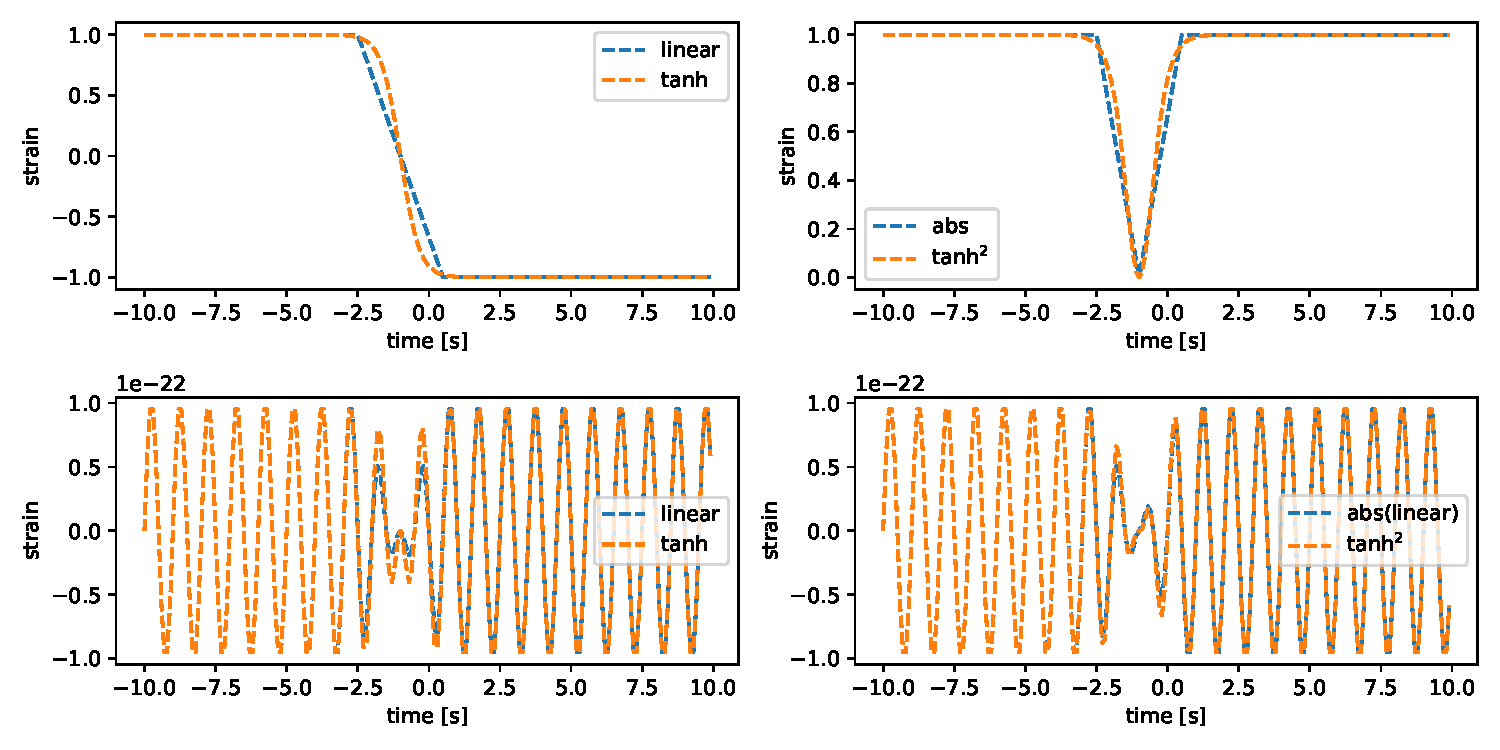
\includegraphics[width=0.7\textwidth, angle=0]{images/Data_analysis/results/envel.pdf}
\captionsetup{width=0.8\textwidth}
\caption[Finite monochromatic waves with an amplitude minimum]{Finite monochromatic waves with an amplitude minimum. Envelopes models \ref{tanh2}, \ref{tanh}, \ref{line} acting on a monochormatic wave with parameters $f=1$ Hz, $d=20$ s, $t_{0}=-10$ s with a zero crossing at -1s.}
\label{env.ex}
\end{center}
\end{figure}
\FloatBarrier


The following is going to be a brief qualitative study for postmerger waveforms generated by non-spinning equal mass and spinning equal mass BNS systems using models \ref{line}, \ref{tanh}, and \ref{tanh2}. The analysis will further examine whether the SNR recovery or parameter estimation improves compared to the results obtained with the constant amplitude model \ref{eq:20}.


\subsection*{Findings}

Let us begin by considering a postmerger waveform generated by a non-spinning Equal mass BNS system. The SNR \ref{pul} is computed in a 3-dimensional 80x80x20 cubic mesh, where the frequency ranges between 2000-2500Hz, and the duration from 5ms to $1.5\cdot d_{postm}$ (see equation \ref{dp}). The width dimension ranges between 1 and 10 ms.

The results obtained using the linear zero-crossing model \ref{line} show us a marginally different SNR recovery as in figure \ref{eqmass} while having an accurate estimation of the waveform's main frequency, duration, and width of the zero-crossing region.

\begin{figure}[hbt!]
\begin{center}
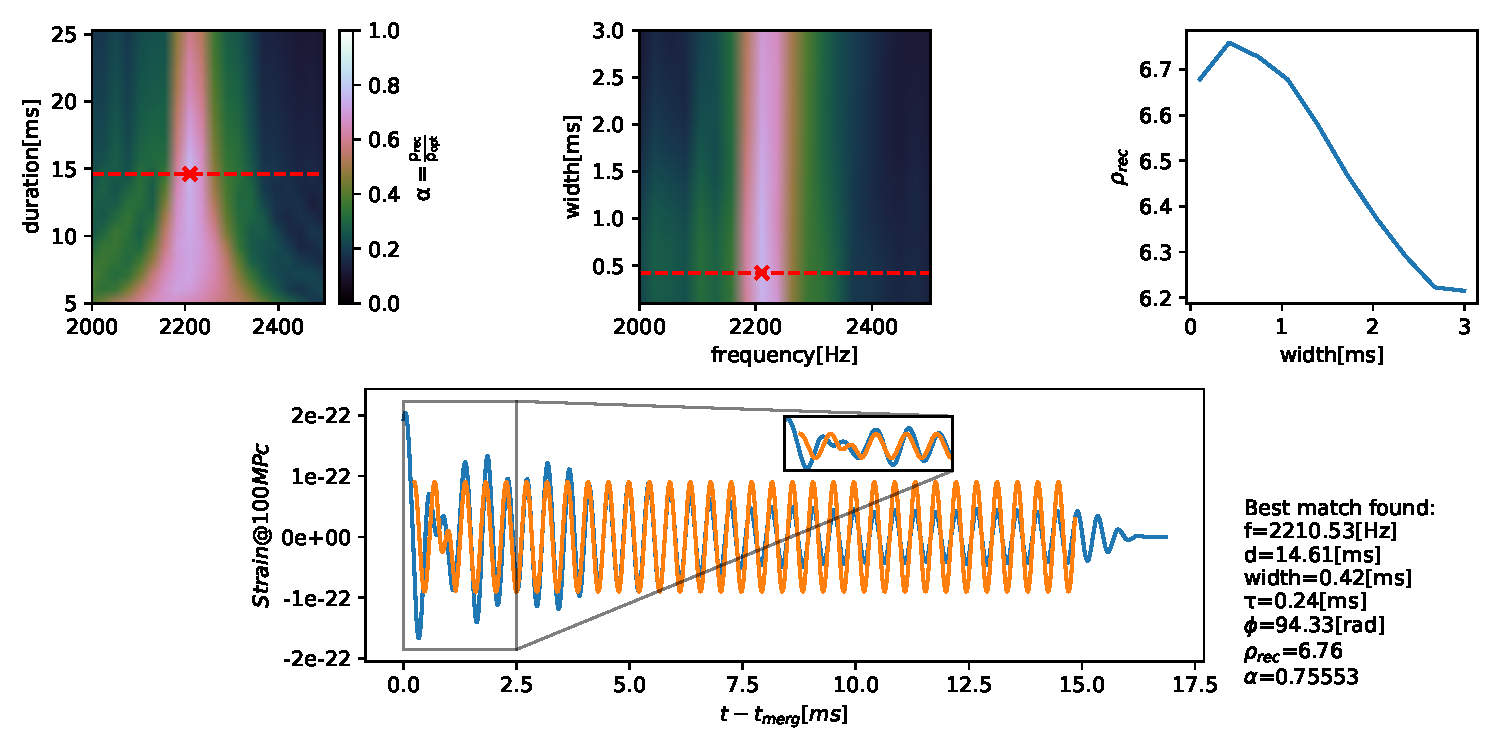
\includegraphics[width=\textwidth, angle=0]{images/Data_analysis/results/envel_35_lin.pdf}
\captionsetup{width=0.8\textwidth}
\caption[Linear zero-crossing envelope model matching an equal mass BNS postmerger waveform]{Linear zero-crossing envelope model matching an equal mass BNS postmerger waveform. This plot shows the duration-frequency, width-frequency, and width-$\rho_{rec}$ planes to depict how the SNR recovery along all dimensions of the model \ref{line}. The best matching template and the waveform BAM:0035:R01 of the CoRe BNS catalog \cite{Dietrich:2018phi} are plotted in the bottom panel.}
\end{center} 
\end{figure}

\FloatBarrier

In addition, compared with the than constant amplitude case shown in figure \ref{eqmass}, the hyperbolic tangent model \ref{tanh} shows us a worse SNR recovery, while improving the postmerger's duration estimation.

\begin{figure}[hbt!]
\begin{center}
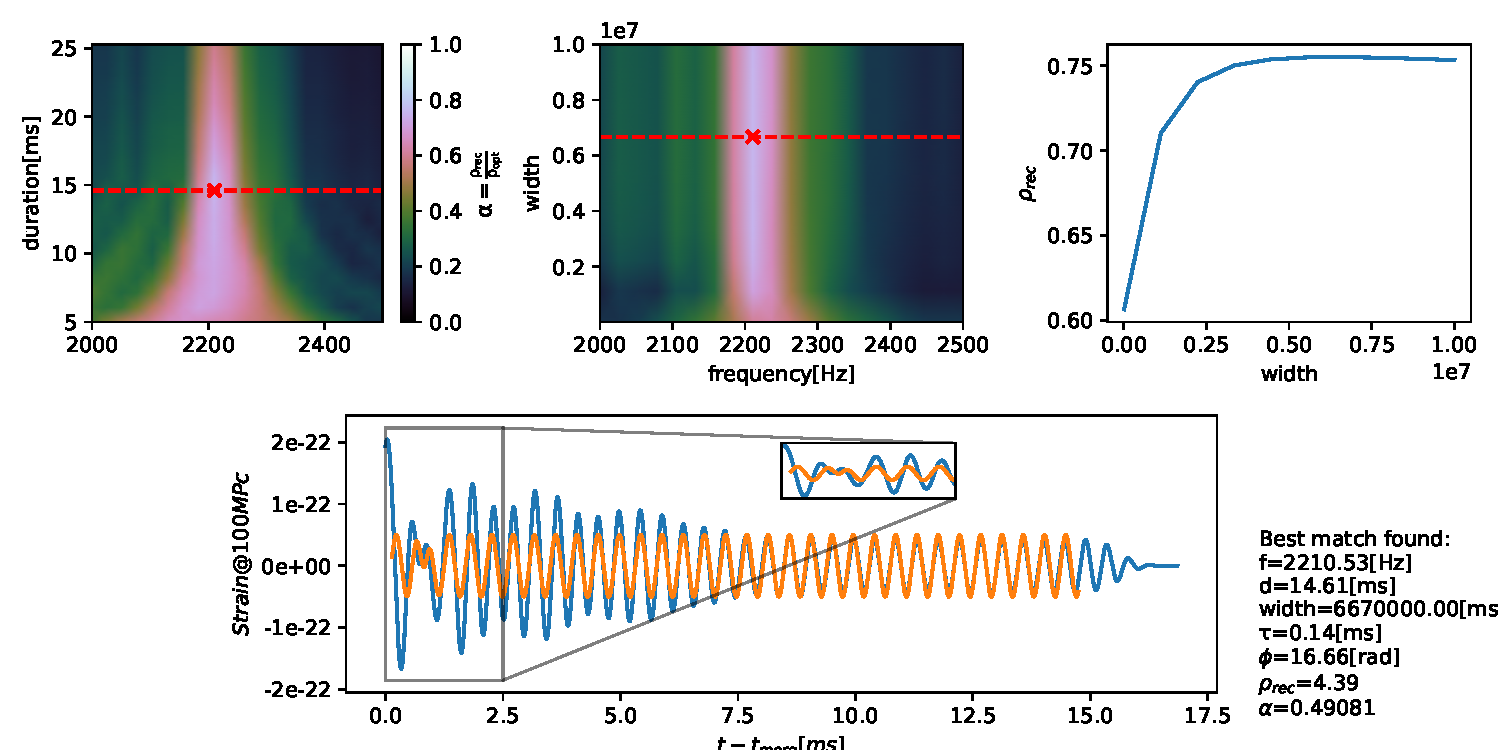
\includegraphics[width=\textwidth, angle=0]{images/Data_analysis/results/envel_35_tanh.pdf}
\captionsetup{width=0.8\textwidth}
\caption[Zero-crossing $tanh$ envelope model matching an equal mass BNS postmerger waveform]{Zero-crossing $tanh$ envelope model matching an equal mass BNS postmerger waveform. This plot shows the duration-frequency, width-frequency, and width-$\rho_{rec}$ planes to depict how the SNR recovery along all dimensions of the model \ref{tanh}. The best matching template and the waveform BAM:0035:R01 of the CoRe BNS catalog \cite{Dietrich:2018phi} are plotted in the bottom panel.}
\end{center}
\end{figure}

\FloatBarrier

Finally, compared to the model \ref{tanh}, we can observe that the quadratic hyperbolic tangent model \ref{tanh2} shows us a worse SNR recovery, duration, and width estimation for this type of waveform.

\begin{figure}[hbt!]
\begin{center}
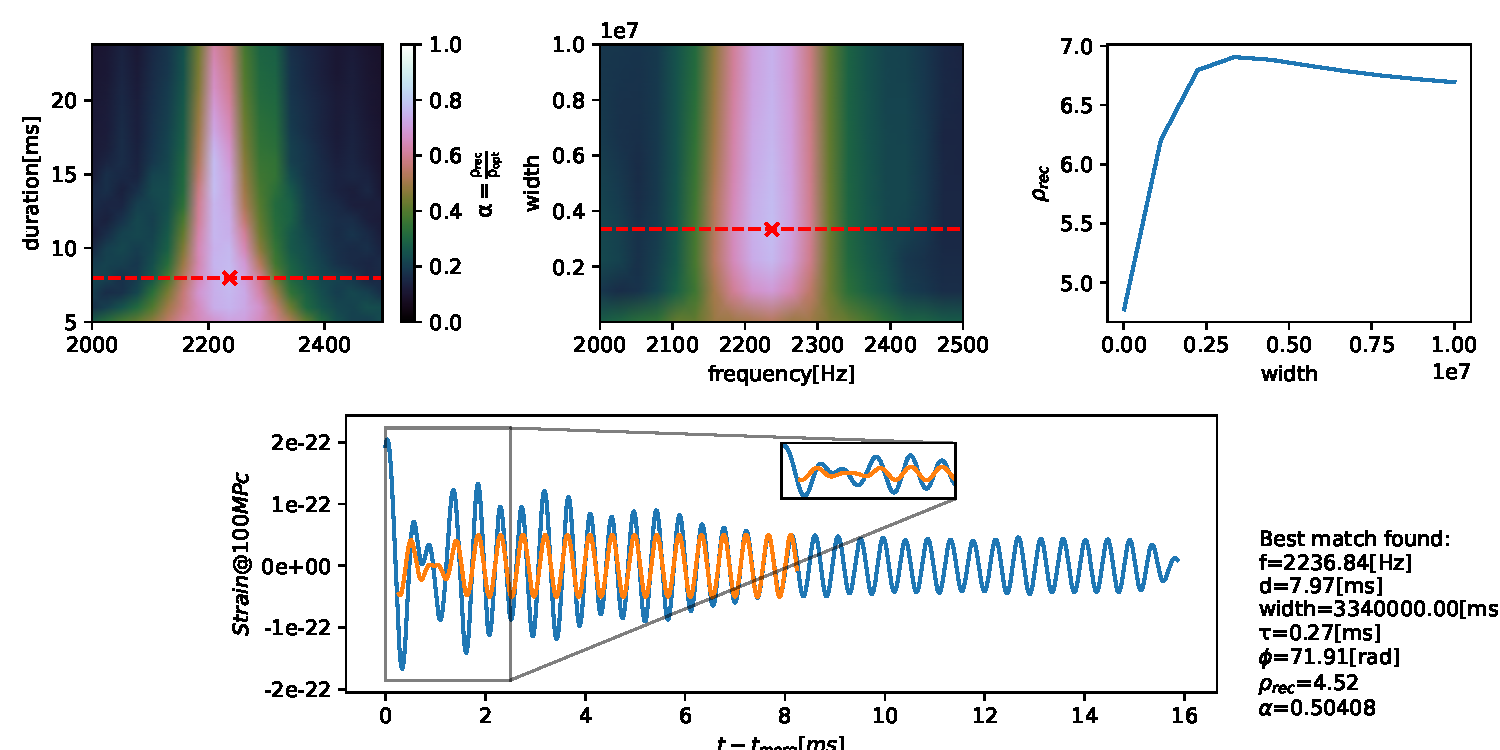
\includegraphics[width=\textwidth, angle=0]{images/Data_analysis/results/envel_35_tanh2.pdf}
\captionsetup{width=0.8\textwidth}
\caption[Zero-crossing $tanh^2$ envelope model matching an equal mass BNS postmerger waveform]{Zero-crossing $tanh^2$ envelope model matching an equal mass BNS postmerger waveform. This plot shows the duration-frequency, width-frequency, and width-$\rho_{rec}$ planes to depict how the SNR recovery along all dimensions of the model \ref{tanh2}. The best matching template and the waveform BAM:0035:R01 of the CoRe BNS catalog \cite{Dietrich:2018phi} are plotted in the bottom panel.}
\end{center}
\end{figure}

\FloatBarrier

\newpage
Moreover, we observe improvements in parameter estimation compared to the case shown in figure \ref{spi} for the following example waveform generated by a highly spinning BNS. The linear model \ref{line} improves the duration recovery compared to what was obtained in figure \ref{spi},  but the width parameter is not accurately reconstructed.

\begin{figure}[hbt!]
\begin{center}
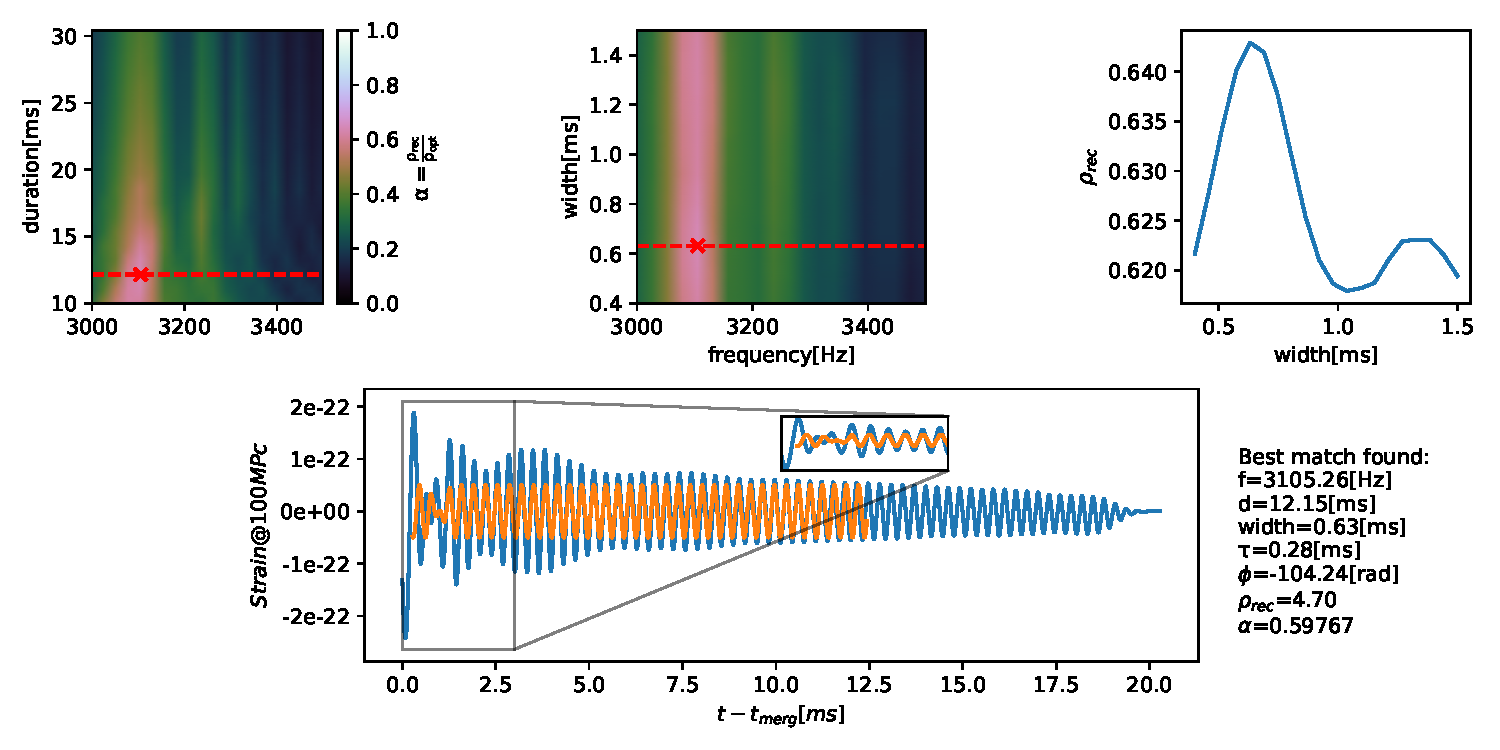
\includegraphics[width=\textwidth, angle=0]{images/Data_analysis/results/envel_110_lin.pdf}
\captionsetup{width=0.8\textwidth}
\caption[Linear zero-crossing envelope model matching a spinning BNS postmerger waveform]{Linear zero-crossing envelope model matching an spinning BNS postmerger waveform. This plot shows the duration-frequency, width-frequency, and width-$\rho_{rec}$ planes to depict how the SNR recovery along all dimensions of the model \ref{line}. The best matching template and the waveform BAM:0106:R01 of the CoRe BNS catalog \cite{Dietrich:2018phi} are plotted in the bottom panel.}
\end{center}
\end{figure}

\FloatBarrier

The hyperbolic tangent model \ref{tanh} shows similar duration estimation but gets out of phase around the amplitude minimum.

\begin{figure}[hbt!]
\begin{center}
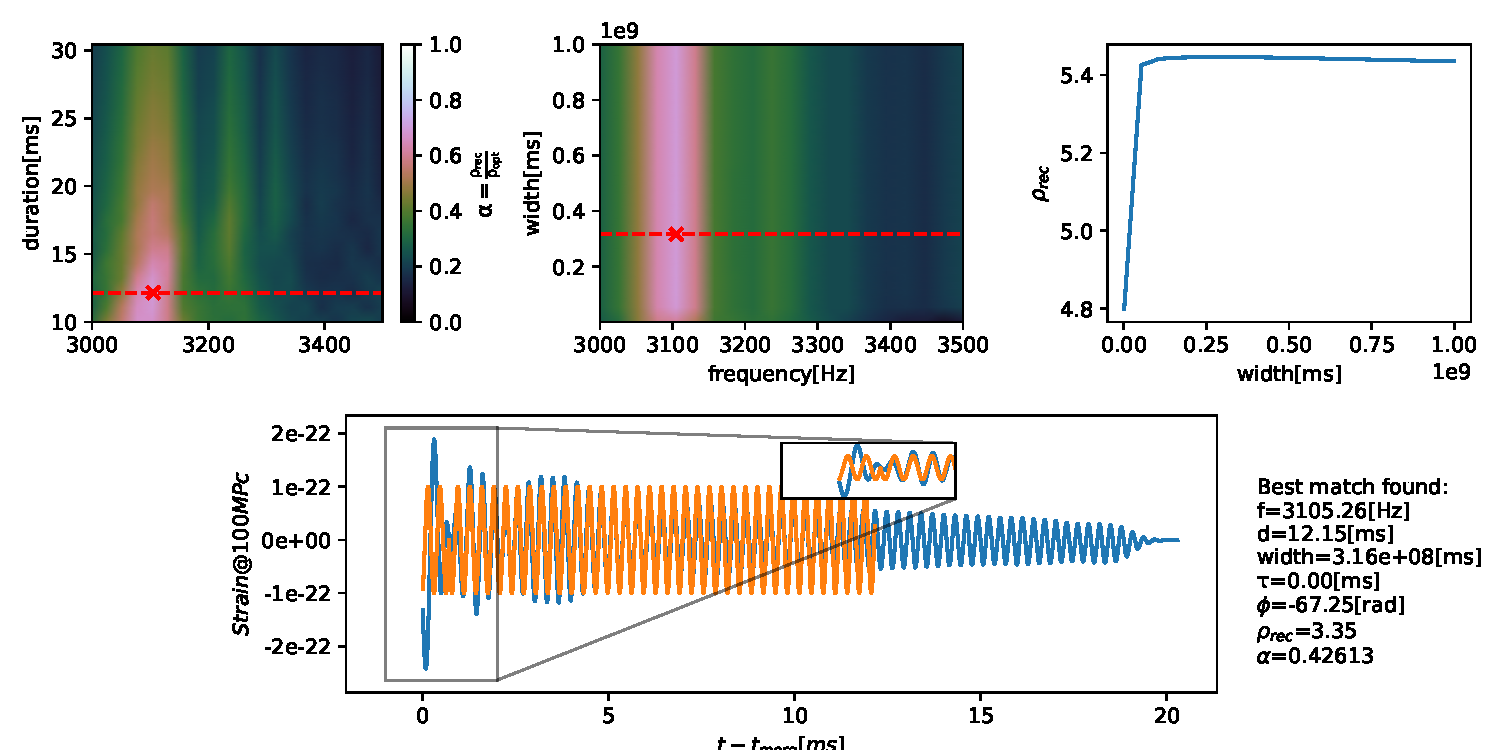
\includegraphics[width=\textwidth, angle=0]{images/Data_analysis/results/envel_110_tanh.pdf}
\captionsetup{width=0.8\textwidth}
\caption[Zero-crossing $tanh$ envelope model matching a spinning BNS postmerger waveform]{Zero-crossing $tanh$ envelope model matching an equal mass BNS postmerger waveform. This plot shows the duration-frequency, width-frequency, and width-$\rho_{rec}$ planes to depict how the SNR recovery along all dimensions of the model \ref{tanh}. The best matching template and the waveform BAM:0106:R01 of the CoRe BNS catalog \cite{Dietrich:2018phi} are plotted in the bottom panel.}
\end{center}
\end{figure}

\FloatBarrier
\newpage
The quadratic hyperbolic tangent model \ref{tanh2} reproduces, in this case, much better the postmerger phase around the amplitude minimum while improving the duration estimation, compared to the constant amplitude model seen in figure \ref{spi}.

\begin{figure}[hbt!]
\begin{center}
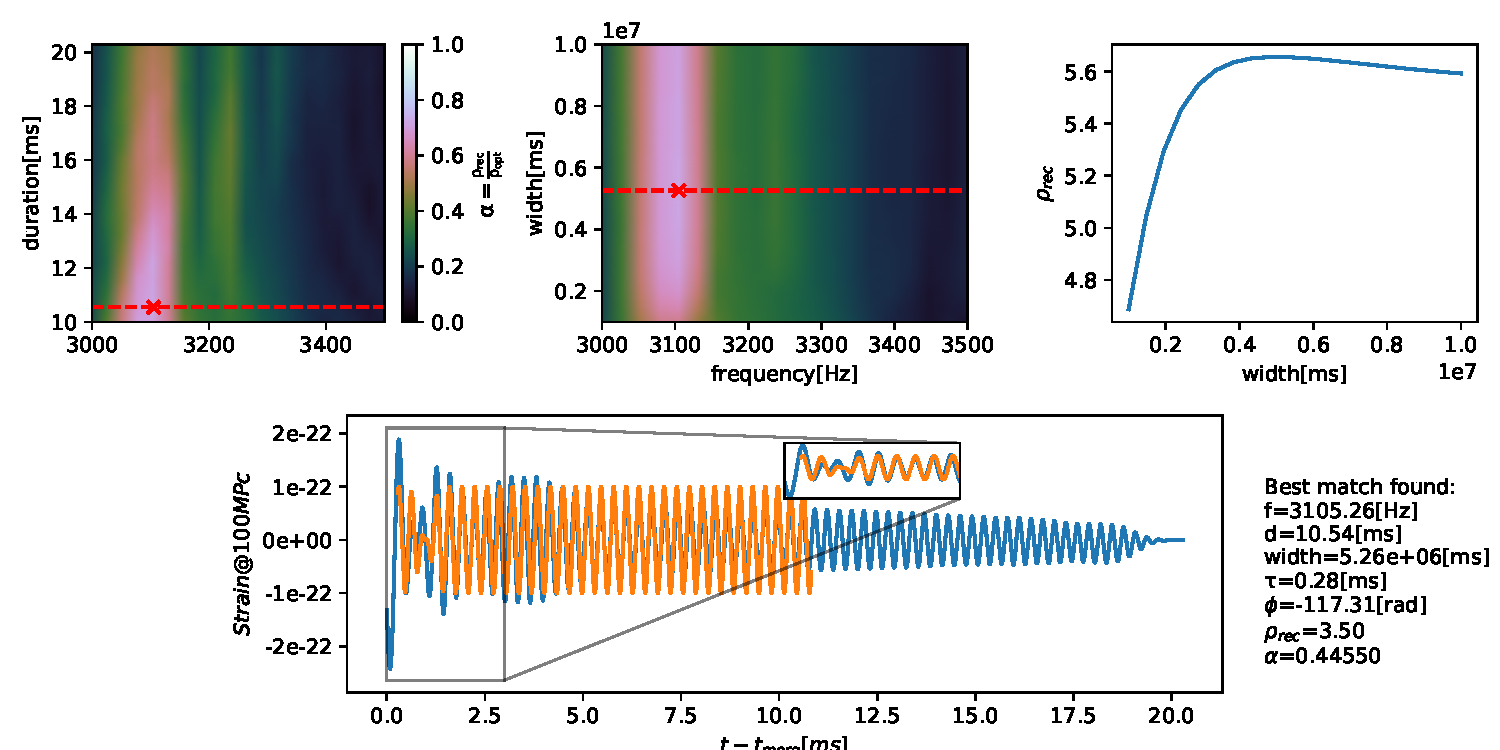
\includegraphics[width=\textwidth, angle=0]{images/Data_analysis/results/envel_110_tanh2.pdf}
\captionsetup{width=0.8\textwidth}
\caption[Zero-crossing $tanh^2$ envelope model matching a spinning BNS postmerger waveform]{Zero-crossing $tanh^2$ envelope model matching an equal mass BNS postmerger waveform. This plot shows the duration-frequency, width-frequency, and width-$\rho_{rec}$ planes to depict how the SNR recovery along all dimensions of the model \ref{tanh2}. The best matching template and the waveform BAM:0106:R01 of the CoRe BNS catalog \cite{Dietrich:2018phi} are plotted in the bottom panel.}
\end{center}
\end{figure}

\FloatBarrier





\section{Impacts of amplitude and phase evolution on different postmerger  waveforms}

In general, expecting a simple monochromatic model to match perfectly every possible postmerger BNS phase sounds optimistic. As we saw in the previous section, adding simple features to improve parameter estimation accuracy may lead to SNR losses or only marginal improvements when running the matched filtering algorithm at the cost of increasing the dimensionality of the model's parameter space.

The following section proposes a method that implicitly evaluates two possible paths for creating future simple  BNS postmerger waveform approximants. To carry out such a task, we will take the complex strain \ref{fvr} of all waveforms shown in section \ref{2dsearch} and its amplitude envelopes $|H(t)|$, phases $\phi(t)=\angle H(t)$, and durations \ref{dp} to build the following template models:

\begin{itemize}[leftmargin=*]
\item A wave with constant amplitude and perfect phase evolution.

\begin{equation}\label{pha-evol}
g(t) = \cdot \begin{cases} 
      0 &, t< t_{merg} \\
      A \cdot sin(\phi(t)) &, t_{merg} \leq t \leq t_{merg} + d_{postm} \\
      0 &, t> t_{merg} + d_{postm}
   \end{cases}
\end{equation}


\item A monochromatic wave with perfect amplitude evolution.

\begin{equation}\label{a-evol}
f(t) = |H(t)| \cdot \begin{cases} 
      0 &, t< t_{merg} \\
      sin(2\pi f_{_{best}}\cdot t + \phi_{opt}) &, t_{merg} \leq t \leq t_{merg} + d_{postm} \\
      0 &, t> t_{merg} + d_{postm}
   \end{cases}
\end{equation}

\end{itemize}


The SNR envelope as a function of the timeshift will be computed by overlapping for the functions \ref{a-evol}, \ref{pha-evol}, \ref{eq:20} against each waveform $H(t)$ as shown in figure \ref{fig:7}. Finally, the maximum of each SNR curve will be compared with the optimum one obtained by overlapping the waveform $H(t)$ with itself. In this way, for each type of waveform, it will be evaluated if a model like \ref{a-evol} could be closer to the optimal SNR recovery than the model \ref{pha-evol} or vice versa.

In the following figure, we show how for an example waveform, we generate three different templates and SNR curves: a constant amplitude monochromatic wave (yellow), a wave built using the model \ref{pha-evol}(red), and wave built using model \ref{a-evol} (black). We compare all SNR curves with the one produced by overlapping the waveform with itself (blue).

\begin{figure}[hbt!]
\begin{center}
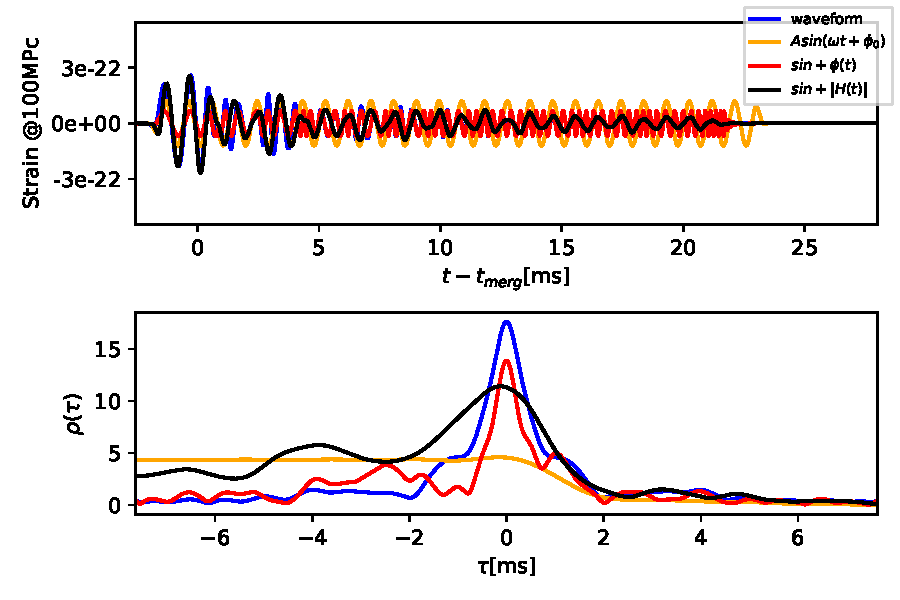
\includegraphics[width=\textwidth, angle=0]{images/Data_analysis/results/phi-A0.pdf}
\captionsetup{width=0.8\textwidth}
\caption[Modelling waveform with a strange amplitude modulation from the CoRe catalog]{Modelling waveform with a strange amplitude modulation from the CoRe catalog. This figure shows the waveform BAM:0027(top) \cite{Dietrich:2018phi} being overlapped with a monochromatic template with constant amplitude and frequency (yellow), a template created using the model \ref{pha-evol} (red), a template created using the model \ref{a-evol} (black), and itself (blue). The SNR curves as a function of timeshift are shown in the bottom panel.}
\label{analysis}
\end{center}
\end{figure}
\FloatBarrier



\subsubsection*{Postmerger waveforms with rectangular windowing}


In the following figure, shows the an equal mass waveform (top), a high mass ratio waveform (mid), and a spinning waveform(bottom) on the left and the SNR results are computed on the right as described for the case shown in figure \ref{analysis}.


\begin{figure}[hbt!]
\begin{center}
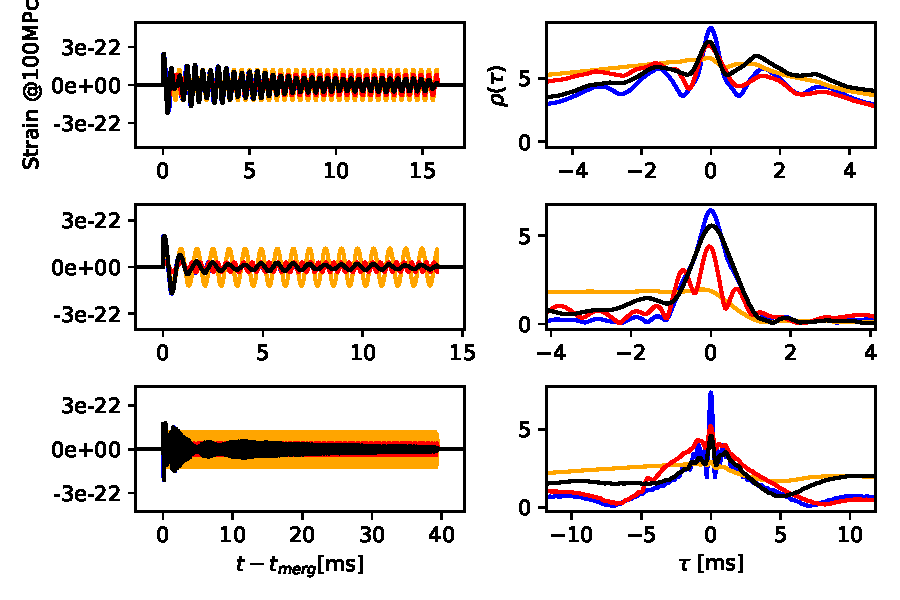
\includegraphics[width=0.7\textwidth, angle=0]{images/Data_analysis/results/phi-A1.pdf}
\captionsetup{width=0.8\textwidth}
\caption[Future simple postmerger models for $q=1$, $q>1.6$ and $\chi_{_{eff}}>0.2$ waveforms]{Future simple postmerger models for $q=1$, $q>1.6$ and $\chi_{_{eff}}>0.2$ waveforms. This image shows the time domain representations of an equal mass waveform (top), a high mass ratio waveform (mid), and a highly spinning waveform (bottom). Their respective overlaps as a function of timeshift against the models \ref{eq:20}, \ref{a-evol}, and \ref{pha-evol} are shown in front of each waveform using the same coloring scheme as in figure \ref{analysis}.}
\label{ncfrnv}
\end{center}
\end{figure}
\FloatBarrier

In addition, the following SNR curves are also computed for a wavefor generated by a heavy BNS system (top), a highly eccentric waveform (mid) and a waveform generated by a BNS where viscous hydrodynamics were considered (bottom).

\begin{figure}[hbt!]
\begin{center}
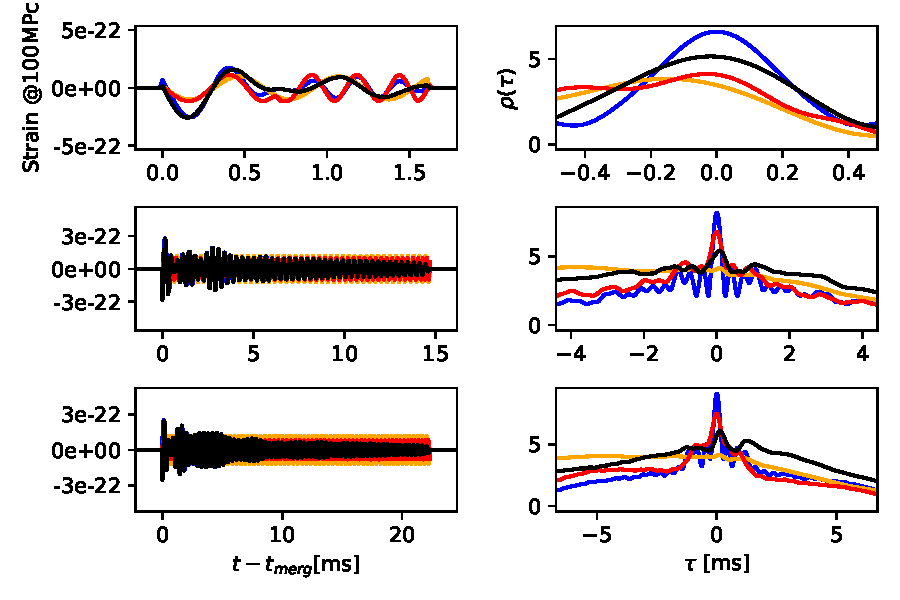
\includegraphics[width=0.7\textwidth, angle=0]{images/Data_analysis/results/phi-A2.pdf}
\captionsetup{width=0.8\textwidth}
\caption[Future simple postmerger models for $\delta>1.6$, $e>0.4$, and a waveform with viscous hydrodynamics waveforms]{Future simple postmerger models for $\delta>1.6$, $e>0.4$, and a waveform with viscous hydrodynamics waveforms. This image shows the time domain representations of a short BNS waveform (top), a highly eccentric waveform (mid), and an equal mass waveform with strong amplitude modulation (bottom). Their respective overlaps as a function of timeshift against the models \ref{eq:20}, \ref{a-evol}, and \ref{pha-evol} are shown in front of each waveform using the same coloring scheme as in figure \ref{analysis}.}
\label{ncejn}
\end{center}
\end{figure}
\FloatBarrier


The following table is shown to compare quantitatively the maximum recovered SNR for all models after being overlapped against all waveforms shown in section \ref{2dsearch}. The first column shows the simulation ID, the second row shows the optimal SNR \ref{sopt} computed for that waveform at 100 MPc, the third column shows the maximum recovered SNR using the constant amplitude model \ref{eq:20} denoted by $\alpha(\phi_{const.})$, the fourth column the recovery using the model \ref{pha-evol} denoted by $\alpha(\phi(t))$, and the fifth column the recovery when using the model \ref{a-evol} denoted by $\alpha(|H(t)|)$.

Notice how the high mass ratio waveforms and waveforms generated by heavy BNS systems prefer the model with perfect amplitude evolution \ref{a-evol}, while other waveforms get closer to the optimal SNR when overlapped against model \ref{pha-evol}.


\begin{table}[!htbp]
\begin{center}

\begin{tabular}{ccccc}

simulation&$S_{opt}$&$\alpha(\phi_{const.})$&$\alpha(\phi(t))$&$\alpha(|H(t)|)$\\ 
\hline\\ 
$\mathrm{{q=1}_{_{_{(BAM:0035)}}}}$&8.943&0.734&0.841&0.875\\  
$\mathrm{{q>1.6}_{_{_{(BAM:0021)}}}}$&6.429&0.293&0.679&0.863\\  
$\mathrm{{X_{eff}>0.2}_{_{_{(BAM:0110)}}}}$&7.350&0.398&0.707&0.622\\  
$\mathrm{{\delta>1.6}_{_{_{(BAM:0011)}}}}$&6.607&0.535&0.611&0.778\\  
$\mathrm{{e>0.4}_{_{_{(BAM:0114)}}}}$&8.186&0.515&0.827&0.646\\  
$\mathrm{{visc.\hspace{1mm} HD}_{_{_{(THC:0019)}}}}$&9.122&0.461&0.819&0.638\\  
\hline\\ 
\end{tabular}
\captionsetup{width=0.8\textwidth}
\caption[Improved simple modelling summary for a rectangular window function]{Improved simple modelling summary for a rectangular window function. This table summarizes the SNR recovery with the Einstein telescope at 100MPc for the models \ref{pha-evol}, \ref{a-evol}, and \ref{eq:19} on all waveform examples shown in section \ref{2dsearch} when using a rectangular window function to define the postmerger phase the BNS waveform.}
\label{table untapered}
\end{center}
\end{table}
\FloatBarrier

%Notice that  how the model with perfect amplitude evolution (black) gets closer to the optimal curve (blue) the high mass ratio waveforms(mid row). For the other two waveform all models show marginal differences where the model with perfect phase evolution is preferred (red).




\subsubsection*{Tapered postmerger: Impacts of spectral leakage}

In what follows we discuss whether the presence of the hard cutoff introduced by the rectangular window causes spectral leakage when computing FFTs that affect the relative height of the SNR peaks shown in figures \ref{ncejn}, \ref{ncfrnv} with respect to the optimal SNR curve in blue. The following plots are computed following as in the example shown in figure \ref{analysis}. However we will allow, on all waveforms shown in figures \ref{ncejn} and \ref{ncfrnv}, a few cycles before merger time and taper the signal using a Tukey window of parameter n=0.1 (see \cite{bloomfield1976fourier}).


\begin{figure}[hbt!]
\begin{center}
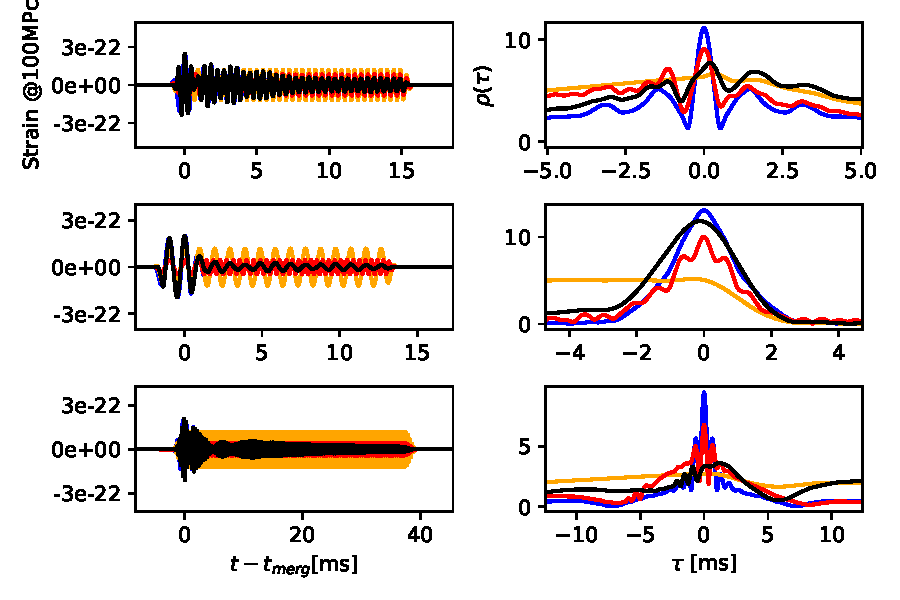
\includegraphics[width=0.7\textwidth, angle=0]{images/Data_analysis/results/phi-A3.pdf}
\captionsetup{width=0.8\textwidth}
\caption[Tapered partial modeling for $q=1$, $q>1.6$ and $\chi{eff}>0.2$ waveforms]{This image shows the time domain representations of all models(left) and their respective overlaps as a function of timeshift(right). Colors follow the same pattern described in figure \ref{analysis}. The top waveform belongs to an equal mass system $q=1$, the one in the middle panel is a high mass ratio waveform $q>1.5$, and the lower panel shows a spinning waveform$\chi_{eff}>0.2$.}
\end{center}
\end{figure}
\FloatBarrier

\begin{figure}[hbt!]
\begin{center}
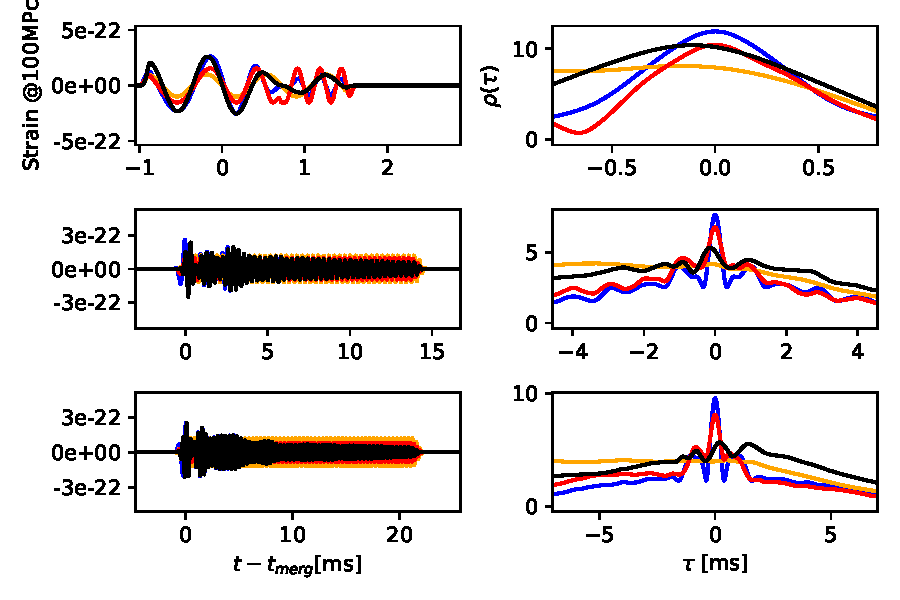
\includegraphics[width=0.7\textwidth, angle=0]{images/Data_analysis/results/phi-A4.pdf}
\captionsetup{width=0.8\textwidth}
\caption[Tapered partial modeling for $\delta>1.6$, $e>0.4$, and waveforms with viscous hydrodynamics effects]{Tapered partial modeling for $\delta>1.6$, $e>0.4$, and waveforms with viscous hydrodynamics effects. This image shows the time domain representations of all models(left) and their respective overlaps as a function of timeshift(right). Colors follow the same pattern described in figure \ref{analysis}. The top waveform belongs to a heavy system $\delta>1.6$(see equation \ref{delta}), the one in the middle panel is a highly eccentric waveform $e>0.4$, and the lower panel shows a waveform with viscous hydrodynamics.}
\end{center}
\end{figure}
\FloatBarrier

The following table compares quantitatively the maximum recovered SNR for all models after being overlapped against all waveforms shown in section \ref{2dsearch}. The first column lists all waveforms by simulation ID, and the second row shows the time allowed before the merger time for applying the Tukey window. The third column shows the Tukey parameter n used to taper the waveform, and the last four columns have the same meaning as in table \ref{table untapered}.


Notice how heavy BNS systems generate high mass ratio waveforms, and waveforms get closer to the optimal SNR when using the model with perfect amplitude evolution \ref{a-evol}. On the other hand, the other waveforms benefit more from the perfect phase evolution model \ref{a-evol}.

\begin{table}[!htbp]
\begin{center}

\begin{tabular}{ccccccc}
simulation&time before merger[ms]&n-tukey&$S_{opt}$&$\alpha(\phi_{const.})$&$\alpha(\phi(t))$&$\alpha(|H(t)|)$\\ 
\hline\\ 
$\mathrm{{q=1}_{_{_{(BAM:0035)}}}}$&1.0&0.1&11.132&0.596&0.815&0.654\\  
$\mathrm{{q>1.6}_{_{_{(BAM:0021)}}}}$&2.0&0.1&13.058&0.389&0.766&0.900\\  
$\mathrm{{X_{eff}>0.2}_{_{_{(BAM:0110)}}}}$&2.0&0.1&9.447&0.288&0.718&0.381\\  
$\mathrm{{\delta>1.6}_{_{_{(BAM:0011)}}}}$&1.0&0.1&11.904&0.666&0.876&0.856\\  
$\mathrm{{e>0.4}_{_{_{(BAM:0114)}}}}$&0.5&0.1&7.674&0.550&0.884&0.662\\  
$\mathrm{{visc.\hspace{1mm} HD}_{_{_{(THC:0019)}}}}$&1.0&0.1&9.570&0.436&0.848&0.577\\  
\hline\\ 
\end{tabular}
\captionsetup{width=0.8\textwidth}
\caption[Tapering effects on SNR recovery for $q=1$, $q>1.6$ and $\chi_{_{eff}}>0.2$ waveforms]{Tapering effects on SNR recovery for $q=1$, $q>1.6$ and $\chi_{_{eff}}>0.2$ waveforms. This table summarizes the analysis results for all models when tapering the waveform using a Tukey window to get the postmerger oscillations. It lists the  SNR  recovery results with the Einstein telescope at 100MPc, the second column gives(roughly) the time before maximum amplitude(merger) that allowed the window,  the third column tells the Tukey parameter used, and the last four columns represent the same kind of data shown in table \ref{table untapered}.}
\end{center}
\end{table}
\FloatBarrier





\newpage
\addcontentsline{toc}{part}{Conclusions}

\chapter*{Conclusions}

Modeling the postmerger BNS GW signal is a very interesting open problem. Future detectors being much more sensitive in the kHz band will require the community to have calibrated phenomenological models for the whole BNS signal for the next decade. Future improvements on current phenomenological models and advances in universal and quasi-universal relations help reduce the number of parameters a model would require since they could be inferred from the inspiral or other observations.

This thesis explored the possibility of simple modeling on every waveform in available catalogs, and it complemented those results by addressing whether amplitude or phase evolution modeling could be prioritized separately depending on the source. 
 
The initial analysis showed how the finite monochromatic model performed well on equal mass waveforms and precessing waveforms with only one amplitude minimum. It recovered from 60 to 80\% of the optimal SNR because their waveforms do not have substantial variations in the phase or phase velocity nor significant amplitude variations that could account for phaseshifts of the order of $\pi$ radians. Some sources are above the imposed threshold for detection, and implementing a model with constant amplitude but better phase evolution would get more than 80\% of the SNR while recovering all the signal cycles.

Short waveforms with weighted frequencies around 3kHz belong to systems with $\delta=\frac{M}{M_{TOV}} > 1.6$. The simple monochromatic template model recovered from 80-98\% of the optimal SNR, being a reasonably good model for them. However, most of them are not loud enough to be detectable if a source at a distance of 100MPc or more generates them. Nevertheless, closer sources like GW170817 could have detectable postmerger phases by third-generation detectors.

High mass ratio and highly eccentric waveforms are the best candidates for detection at 100MPc or more. They feature a few loud oscillations after maximum amplitude that contain 60 to 95\% followed by a lower amplitude tail. The transition from the high amplitude initial part to the low amplitude tail looks pretty challenging to recover with a Monochromatic template model because the matched filtering algorithm would not gain much SNR by considering a longer wave. A better amplitude evolution would change this, significantly improving the SNR gains while recovering the low amplitude tail much better.


%Amplitude modeling is more important for short signals generated by systems with a total gravitational mass greater than 1.6  times the maximum TOV mass and waveforms generated by systems with a high mass ratio greater than 1.6. On the other hand, signals generated by equal mass non-spinning binaries and spinning binaries with only one deep strain minimum in the time domain are already well recovered by a monochromatic signal. However, they would significantly improve if one provides a model with a much better phase evolution.




 








